% Generated fragments require trusted human review before compilation.
% This binder never requests shell escape or runs external tools.
\documentclass[11pt]{article}
% Trusted shared apparatus. Requires LuaLaTeX; never use shell escape.
\usepackage{fontspec}
\defaultfontfeatures{Ligatures=TeX}
\IfFontExistsTF{Noto Serif}{\setmainfont{Noto Serif}}{%
  \IfFontExistsTF{DejaVu Serif}{\setmainfont{DejaVu Serif}}{%
    \IfFontExistsTF{Times New Roman}{\setmainfont{Times New Roman}}{%
      \PackageError{gelfand-binder}{No configured Cyrillic serif font installed}{Install Noto Serif or DejaVu Serif, or select an installed Cyrillic font.}%
    }%
  }%
}
\IfFontExistsTF{Noto Sans}{\setsansfont{Noto Sans}}{%
  \IfFontExistsTF{DejaVu Sans}{\setsansfont{DejaVu Sans}}{\setsansfont{Arial}}%
}
\IfFontExistsTF{Noto Sans Mono}{\setmonofont{Noto Sans Mono}}{%
  \IfFontExistsTF{DejaVu Sans Mono}{\setmonofont{DejaVu Sans Mono}}{\setmonofont{Courier New}}%
}
\usepackage[a4paper,margin=22mm]{geometry}
\usepackage{amsmath,amssymb,amsthm,mathtools}
\usepackage{xcolor}
\usepackage{tikz}
\usepackage{tikz-cd}
\usetikzlibrary{arrows.meta,positioning,calc}
\usepackage{hyperref}
\hypersetup{unicode=true,colorlinks=true,linkcolor=blue,pdftitle={Gelfand transcription binder}}
\newtheorem{theorem}{Theorem}
\newtheorem{lemma}{Lemma}
\newtheorem{proposition}{Proposition}
\newtheorem{corollary}{Corollary}
\theoremstyle{definition}
\newtheorem{definition}{Definition}
\newtheorem{example}{Example}
\theoremstyle{remark}
\newtheorem{remark}{Remark}
\setlength{\parindent}{0pt}
\setlength{\parskip}{0.55em}
\setlength{\emergencystretch}{3em}
\newcommand{\SourcePage}[2]{%
  \clearpage\phantomsection\label{#1:source-page}%
  \addcontentsline{toc}{subsection}{#1}%
  {\small\sffamily\color{blue!60!black}Source scan frame: #1; visible page/leaf label: #2}\par\medskip%
}
\newcommand{\Unclear}[3]{%
  \begingroup\color{orange!70!black}%
  [Unresolved reading #1/#2: #3]\endgroup%
}
\newcommand{\Incomplete}[3]{%
  \par\begingroup\color{red!65!black}\textbf{Incomplete #1/#2:} #3\endgroup\par%
}
\newcommand{\SourceFigure}[3]{%
  \par\begingroup\color{blue!60!black}\textbf{\hyperref[#1:source-page]{Source figure #1/#2}:} #3%
  \par\textit{Consult the authoritative scan at this locator.}\endgroup\par%
}



% Reader layout only. Original diplomatic text is retained verbatim.
\setlength{\parskip}{0.35em}
\setlength{\emergencystretch}{4em}
\renewcommand{\SourcePage}[2]{%
  \par\addvspace{1em}\phantomsection\label{#1:source-page}%
  \addcontentsline{toc}{subsection}{#1}%
  {\footnotesize\sffamily\color{blue!55!black}#1%
    \def\givenlabel{#2}\def\nolabel{unlabelled}%
    \ifx\givenlabel\nolabel\else\quad[номер в источнике: #2]\fi
  }\par\nobreak\smallskip%
}
\renewcommand{\Unclear}[3]{%
  \begingroup\color{orange!65!black}%
  \ifmmode\text{[неясно: #3]}\else[неясно: #3]\fi\endgroup%
}
\renewcommand{\Incomplete}[3]{%
  \par\begingroup\color{red!60!black}\textbf{Неразобранный фрагмент:} #3%
  \endgroup\par%
}
\renewcommand{\SourceFigure}[3]{%
  \par\begingroup\color{blue!55!black}\textbf{Рисунок:} #3%
  \par{\small\textit{Исходный рисунок: \hyperref[#1:source-page]{#1}, #2.}}%
  \endgroup\par%
}
\hypersetup{pdftitle={Семинар И. М. Гельфанда. Дипломатическая транскрипция},pdfauthor={},pdfsubject={Русское рабочее издание с отмеченными сомнительными чтениями}}

\usepackage[normalem]{ulem}
\usepackage{newunicodechar}
\usepackage{adjustbox}
\newfontfamily\SourceSymbolFont{Segoe UI Symbol}
\newfontfamily\SourceCJKFont{MS Gothic}
\let\DiplomaticMathUnderline\underline
\renewcommand{\underline}[1]{\ifmmode\DiplomaticMathUnderline{#1}\else\uline{#1}\fi}
\newunicodechar{→}{\ifmmode\text{{\SourceSymbolFont\char"2192}}\else{\SourceSymbolFont\char"2192}\fi}
\newunicodechar{⇒}{\ifmmode\text{{\SourceSymbolFont\char"21D2}}\else{\SourceSymbolFont\char"21D2}\fi}
\newunicodechar{∀}{\ifmmode\text{{\SourceSymbolFont\char"2200}}\else{\SourceSymbolFont\char"2200}\fi}
\newunicodechar{∂}{\ifmmode\text{{\SourceSymbolFont\char"2202}}\else{\SourceSymbolFont\char"2202}\fi}
\newunicodechar{∈}{\ifmmode\text{{\SourceSymbolFont\char"2208}}\else{\SourceSymbolFont\char"2208}\fi}
\newunicodechar{∌}{\ifmmode\text{{\SourceSymbolFont\char"220C}}\else{\SourceSymbolFont\char"220C}\fi}
\newunicodechar{√}{\ifmmode\text{{\SourceSymbolFont\char"221A}}\else{\SourceSymbolFont\char"221A}\fi}
\newunicodechar{∞}{\ifmmode\text{{\SourceSymbolFont\char"221E}}\else{\SourceSymbolFont\char"221E}\fi}
\newunicodechar{∧}{\ifmmode\text{{\SourceSymbolFont\char"2227}}\else{\SourceSymbolFont\char"2227}\fi}
\newunicodechar{∩}{\ifmmode\text{{\SourceSymbolFont\char"2229}}\else{\SourceSymbolFont\char"2229}\fi}
\newunicodechar{∪}{\ifmmode\text{{\SourceSymbolFont\char"222A}}\else{\SourceSymbolFont\char"222A}\fi}
\newunicodechar{∫}{\ifmmode\text{{\SourceSymbolFont\char"222B}}\else{\SourceSymbolFont\char"222B}\fi}
\newunicodechar{∴}{\ifmmode\text{{\SourceSymbolFont\char"2234}}\else{\SourceSymbolFont\char"2234}\fi}
\newunicodechar{∼}{\ifmmode\text{{\SourceSymbolFont\char"223C}}\else{\SourceSymbolFont\char"223C}\fi}
\newunicodechar{≈}{\ifmmode\text{{\SourceSymbolFont\char"2248}}\else{\SourceSymbolFont\char"2248}\fi}
\newunicodechar{≠}{\ifmmode\text{{\SourceSymbolFont\char"2260}}\else{\SourceSymbolFont\char"2260}\fi}
\newunicodechar{≤}{\ifmmode\text{{\SourceSymbolFont\char"2264}}\else{\SourceSymbolFont\char"2264}\fi}
\newunicodechar{≥}{\ifmmode\text{{\SourceSymbolFont\char"2265}}\else{\SourceSymbolFont\char"2265}\fi}
\newunicodechar{⊕}{\ifmmode\text{{\SourceSymbolFont\char"2295}}\else{\SourceSymbolFont\char"2295}\fi}
\newunicodechar{⊗}{\ifmmode\text{{\SourceSymbolFont\char"2297}}\else{\SourceSymbolFont\char"2297}\fi}
\newunicodechar{①}{\ifmmode\text{{\SourceSymbolFont\char"2460}}\else{\SourceSymbolFont\char"2460}\fi}
\newunicodechar{②}{\ifmmode\text{{\SourceSymbolFont\char"2461}}\else{\SourceSymbolFont\char"2461}\fi}
\newunicodechar{③}{\ifmmode\text{{\SourceSymbolFont\char"2462}}\else{\SourceSymbolFont\char"2462}\fi}
\newunicodechar{④}{\ifmmode\text{{\SourceSymbolFont\char"2463}}\else{\SourceSymbolFont\char"2463}\fi}
\newunicodechar{Ⓗ}{\ifmmode\text{{\SourceSymbolFont\char"24BD}}\else{\SourceSymbolFont\char"24BD}\fi}
\newunicodechar{〃}{\ifmmode\text{{\SourceCJKFont\char"3003}}\else{\SourceCJKFont\char"3003}\fi}


% Reader revision 3. Annotation wording and candidates remain unchanged.
\setmainfont{NotoSerif-Regular.ttf}[Path=C:/Windows/Fonts/,ItalicFont=NotoSerif-Italic.ttf,BoldFont=NotoSerif-Bold.ttf,BoldItalicFont=NotoSerif-BoldItalic.ttf]
\usetikzlibrary{shapes.geometric,decorations.pathreplacing,decorations.markings,patterns,fit}
\newsavebox{\ReaderAnnotationBox}
\newcommand{\ReaderAnnotation}[1]{%
  \sbox{\ReaderAnnotationBox}{[неясно: #1]}%
  \ifdim\wd\ReaderAnnotationBox>.70\linewidth
    \parbox[t]{.70\linewidth}{\raggedright[неясно: #1]}%
  \else\usebox{\ReaderAnnotationBox}\fi%
}
\ExplSyntaxOn
\cs_new_protected:Npn \reader_unclear_candidate:n #1
 {
  \tl_set:Nx \l_tmpa_tl { \tl_to_str:n {#1} }
  % Text explicitly guarded inside a mathematical candidate remains math-safe.
  \regex_replace_all:nnN { \\(?:text|textrm|textnormal|textbf|operatorname)\s*\{[^{}]*\} } { } \l_tmpa_tl
  \regex_match:nVTF { [\x{0400}-\x{052F}] | \$ } \l_tmpa_tl
   { \ifmmode \text{\ReaderAnnotation{#1}} \else \ReaderAnnotation{#1} \fi }
   {
    \ifmmode
      [\text{неясно:~}#1]
    \else
      \regex_match:nVTF { [_^] | \\ } \l_tmpa_tl
       { \ensuremath{[\text{неясно:~}#1]} }
       { \ReaderAnnotation{#1} }
    \fi
   }
 }
\RenewDocumentCommand \Unclear { m m m }
 { \begingroup\color{orange!65!black}\reader_unclear_candidate:n{#3}\endgroup }
\ExplSyntaxOff
\newsavebox{\ReaderIncompleteBox}
\newcommand{\ReaderIncompleteNote}[1]{%
 \sbox{\ReaderIncompleteBox}{\textbf{Неразобранный фрагмент:} #1}%
 \ifdim\wd\ReaderIncompleteBox>.70\linewidth
  \parbox[t]{.70\linewidth}{\raggedright\textbf{Неразобранный фрагмент:} #1}%
 \else\usebox{\ReaderIncompleteBox}\fi%
}
\renewcommand{\Incomplete}[3]{%
 \ifmmode\text{\color{red!60!black}\ReaderIncompleteNote{#3}}%
 \else\leavevmode\begingroup\color{red!60!black}\ReaderIncompleteNote{#3}\endgroup\fi%
}
% Ragged right avoids stretching long untranslated abbreviations into margins.
\AtBeginDocument{\raggedright}
\newunicodechar{А}{\ifmmode\text{\char"410\relax}\else\char"410\relax\fi}
\newunicodechar{Б}{\ifmmode\text{\char"411\relax}\else\char"411\relax\fi}
\newunicodechar{В}{\ifmmode\text{\char"412\relax}\else\char"412\relax\fi}
\newunicodechar{Г}{\ifmmode\text{\char"413\relax}\else\char"413\relax\fi}
\newunicodechar{Д}{\ifmmode\text{\char"414\relax}\else\char"414\relax\fi}
\newunicodechar{Е}{\ifmmode\text{\char"415\relax}\else\char"415\relax\fi}
\newunicodechar{Ж}{\ifmmode\text{\char"416\relax}\else\char"416\relax\fi}
\newunicodechar{З}{\ifmmode\text{\char"417\relax}\else\char"417\relax\fi}
\newunicodechar{И}{\ifmmode\text{\char"418\relax}\else\char"418\relax\fi}
\newunicodechar{Й}{\ifmmode\text{\char"419\relax}\else\char"419\relax\fi}
\newunicodechar{К}{\ifmmode\text{\char"41A\relax}\else\char"41A\relax\fi}
\newunicodechar{Л}{\ifmmode\text{\char"41B\relax}\else\char"41B\relax\fi}
\newunicodechar{М}{\ifmmode\text{\char"41C\relax}\else\char"41C\relax\fi}
\newunicodechar{Н}{\ifmmode\text{\char"41D\relax}\else\char"41D\relax\fi}
\newunicodechar{О}{\ifmmode\text{\char"41E\relax}\else\char"41E\relax\fi}
\newunicodechar{П}{\ifmmode\text{\char"41F\relax}\else\char"41F\relax\fi}
\newunicodechar{Р}{\ifmmode\text{\char"420\relax}\else\char"420\relax\fi}
\newunicodechar{С}{\ifmmode\text{\char"421\relax}\else\char"421\relax\fi}
\newunicodechar{Т}{\ifmmode\text{\char"422\relax}\else\char"422\relax\fi}
\newunicodechar{У}{\ifmmode\text{\char"423\relax}\else\char"423\relax\fi}
\newunicodechar{Ф}{\ifmmode\text{\char"424\relax}\else\char"424\relax\fi}
\newunicodechar{Х}{\ifmmode\text{\char"425\relax}\else\char"425\relax\fi}
\newunicodechar{Ц}{\ifmmode\text{\char"426\relax}\else\char"426\relax\fi}
\newunicodechar{Ч}{\ifmmode\text{\char"427\relax}\else\char"427\relax\fi}
\newunicodechar{Ш}{\ifmmode\text{\char"428\relax}\else\char"428\relax\fi}
\newunicodechar{Щ}{\ifmmode\text{\char"429\relax}\else\char"429\relax\fi}
\newunicodechar{Ъ}{\ifmmode\text{\char"42A\relax}\else\char"42A\relax\fi}
\newunicodechar{Ы}{\ifmmode\text{\char"42B\relax}\else\char"42B\relax\fi}
\newunicodechar{Ь}{\ifmmode\text{\char"42C\relax}\else\char"42C\relax\fi}
\newunicodechar{Э}{\ifmmode\text{\char"42D\relax}\else\char"42D\relax\fi}
\newunicodechar{Ю}{\ifmmode\text{\char"42E\relax}\else\char"42E\relax\fi}
\newunicodechar{Я}{\ifmmode\text{\char"42F\relax}\else\char"42F\relax\fi}
\newunicodechar{а}{\ifmmode\text{\char"430\relax}\else\char"430\relax\fi}
\newunicodechar{б}{\ifmmode\text{\char"431\relax}\else\char"431\relax\fi}
\newunicodechar{в}{\ifmmode\text{\char"432\relax}\else\char"432\relax\fi}
\newunicodechar{г}{\ifmmode\text{\char"433\relax}\else\char"433\relax\fi}
\newunicodechar{д}{\ifmmode\text{\char"434\relax}\else\char"434\relax\fi}
\newunicodechar{е}{\ifmmode\text{\char"435\relax}\else\char"435\relax\fi}
\newunicodechar{ж}{\ifmmode\text{\char"436\relax}\else\char"436\relax\fi}
\newunicodechar{з}{\ifmmode\text{\char"437\relax}\else\char"437\relax\fi}
\newunicodechar{и}{\ifmmode\text{\char"438\relax}\else\char"438\relax\fi}
\newunicodechar{й}{\ifmmode\text{\char"439\relax}\else\char"439\relax\fi}
\newunicodechar{к}{\ifmmode\text{\char"43A\relax}\else\char"43A\relax\fi}
\newunicodechar{л}{\ifmmode\text{\char"43B\relax}\else\char"43B\relax\fi}
\newunicodechar{м}{\ifmmode\text{\char"43C\relax}\else\char"43C\relax\fi}
\newunicodechar{н}{\ifmmode\text{\char"43D\relax}\else\char"43D\relax\fi}
\newunicodechar{о}{\ifmmode\text{\char"43E\relax}\else\char"43E\relax\fi}
\newunicodechar{п}{\ifmmode\text{\char"43F\relax}\else\char"43F\relax\fi}
\newunicodechar{р}{\ifmmode\text{\char"440\relax}\else\char"440\relax\fi}
\newunicodechar{с}{\ifmmode\text{\char"441\relax}\else\char"441\relax\fi}
\newunicodechar{т}{\ifmmode\text{\char"442\relax}\else\char"442\relax\fi}
\newunicodechar{у}{\ifmmode\text{\char"443\relax}\else\char"443\relax\fi}
\newunicodechar{ф}{\ifmmode\text{\char"444\relax}\else\char"444\relax\fi}
\newunicodechar{х}{\ifmmode\text{\char"445\relax}\else\char"445\relax\fi}
\newunicodechar{ц}{\ifmmode\text{\char"446\relax}\else\char"446\relax\fi}
\newunicodechar{ч}{\ifmmode\text{\char"447\relax}\else\char"447\relax\fi}
\newunicodechar{ш}{\ifmmode\text{\char"448\relax}\else\char"448\relax\fi}
\newunicodechar{щ}{\ifmmode\text{\char"449\relax}\else\char"449\relax\fi}
\newunicodechar{ъ}{\ifmmode\text{\char"44A\relax}\else\char"44A\relax\fi}
\newunicodechar{ы}{\ifmmode\text{\char"44B\relax}\else\char"44B\relax\fi}
\newunicodechar{ь}{\ifmmode\text{\char"44C\relax}\else\char"44C\relax\fi}
\newunicodechar{э}{\ifmmode\text{\char"44D\relax}\else\char"44D\relax\fi}
\newunicodechar{ю}{\ifmmode\text{\char"44E\relax}\else\char"44E\relax\fi}
\newunicodechar{я}{\ifmmode\text{\char"44F\relax}\else\char"44F\relax\fi}
\newunicodechar{Ё}{\ifmmode\text{\char"401\relax}\else\char"401\relax\fi}
\newunicodechar{ё}{\ifmmode\text{\char"451\relax}\else\char"451\relax\fi}

\newunicodechar{æ}{\ifmmode\text{\char"E6\relax}\else\char"E6\relax\fi}
\newunicodechar{−}{\ifmmode\mathbin{\text{\SourceSymbolFont\char"2212\relax}}\else{\SourceSymbolFont\char"2212\relax}\fi}

\begin{document}
\begin{center}
{\Large Семинар И. М. Гельфанда}\par\medskip
{\LARGE Дипломатическая транскрипция}\par\bigskip
{\large Рабочее русское издание}\par\medskip
{\large Том 18 из 34. Архивная глава 018}\par\bigskip
Кадры GELFAND-P000919 -- GELFAND-P000953\par

\end{center}
\medskip
Сокращения, отменённые записи и сомнительные чтения сохранены.
Неразобранные фрагменты отмечены в тексте. Математические утверждения
источника переданы без молчаливых исправлений.

Это рабочее издание: сверка с рукописью продолжается. В текущем комплекте
учтены 1503 из 1527 кадров; 24 кадра пока представлены явными указателями
отсутствующего возврата. Полный журнал чтений и происхождения данных
сохранён в основном рабочем переплёте.

Границы кадров показаны небольшими синими указателями; печатный текст
продолжается без обязательного разрыва страницы после каждого кадра.
\bigskip\hrule\bigskip
\SourcePage{GELFAND-P000919}{unlabelled}
% Original 2441x3481 viewed directly at original detail, including all edges and blank upper field.
% Reviewed crops (x0,y0,x1,y1; enlargement): (100,1250,1270,1840;3x), (110,1820,2350,2470;3x), (90,2450,2380,3000;3x), (100,2960,2270,3470;3x), (440,1670,950,1800;8x), (440,1850,970,1980;8x), (610,2790,1480,2975;6x), (1055,3070,1330,3160;6x), (375,2160,810,2250;8x), (540,2120,645,2260;10x).

\underline{\underline{13.10.80 г.}}

\underline{Сем. Гельфанда.}

\underline{И.М. Гельфанд.} Рассм. уравнение
\begin{equation*}
\text{(1)}\qquad f(z_1,\ldots,z_n;w_1,\ldots,w_n)=0
\end{equation*}

Пример: рассм. д.у. 2-го порядка
\begin{equation*}
\text{(2)}\qquad y''=f(x,y,y')
\end{equation*}
[Над вторым аргументом $y$ зачёркнуто: \Unclear{GELFAND-P000919}{formula-02-cancelled-superscript}{неразборчивый надстрочный знак}.]

Тогда
\begin{equation*}
\text{(3)}\qquad y=\text{\Unclear{GELFAND-P000919}{formula-03-overwritten-function}{$\varphi$}}(x,\xi,\eta)
\end{equation*}
[Знак функции густо исправлен.]

Обратно, если есть сем-во (3), то по нему строится д.у. 2-го пор.

более обще:
\begin{equation*}
\text{(4)}\qquad F(x,y\text{\Unclear{GELFAND-P000919}{formula-04-separator}{$,$}}\xi,\eta)=0
\end{equation*}
Можно рассм. $\xi,\eta$ как точку и строить двойств. дифф. ур-е.

(1) задает $n$-парм. сем-во гиперповерхностей.

(5) \underline{Задача:} найти геометрию, связ. с этим сем-вом.

Можно делать замены переменных. Напр., в ур-и прямых
\begin{equation*}
\text{(6)}\qquad \xi x+\eta y=1
\end{equation*}

(7) \underline{Задача:} как можно узнать, свод. ли сем-во (4) к сем-ву прямых (6).

\underline{Замены:}
\begin{equation*}
\left\{\begin{aligned}
x_1&=u(x,y)\\
y_1&=v(x,y
\end{aligned}\right.
\qquad
\left\{\begin{aligned}
\xi_1&=\varphi(\xi,\eta)\\
\eta_1&=\psi(\xi,\eta)
\end{aligned}\right.
\end{equation*}
\Unclear{GELFAND-P000919}{substitution-missing-parenthesis}{В строке $y_1=v(x,y$ закрывающая скобка не видна.}

(8) \underline{Общее определение:} \underline{двойное расслоение}

(9) элемент — \underline{точка и прох. через него кривая}

(кривые из 2-пар. сем-ва)

\begin{center}
\begin{adjustbox}{max width=\linewidth}
\begin{tikzcd}[column sep=small]
 & A \arrow[dl,"\pi_1"'] \arrow[dr,"\pi_2"] & \\
B & & \Gamma
\end{tikzcd}
\end{adjustbox}

(есть 2 проекции)
\end{center}

(см. ст. \underline{Гельфанд}, \underline{Гиндикин}, \underline{Шапиро} в ФА)

\SourcePage{GELFAND-P000920}{unlabelled}
% Original 2440x3480 viewed directly at original detail, including margins and boundary strips.
% Reviewed crops (x0,y0,x1,y1; enlargement): (100,70,1900,700;3x), (130,680,2020,1210;3x), (140,1190,1740,1830;3x), (130,1810,1380,2570;3x), (140,2570,2300,3080;3x), (160,3040,1600,3340;3x), (1190,360,1650,495;6x), (380,1530,1560,1735;5x), (1790,1830,1960,1980;10x), (830,2690,2240,2870;5x), (670,2860,1990,3065;5x), (1320,2735,1455,2820;10x), (1160,2910,1310,3050;10x), (1085,2890,1245,3070;10x), (385,3050,650,3170;8x), (650,1910,930,2140;8x).

(10) \underline{Требование:} если
\begin{equation*}
\left\{\begin{aligned}
\pi_1x&=\pi_1x'\\
\text{и}\quad\pi_2x&=\pi_2x'
\end{aligned}\right.
,\quad\text{то }x=x'
\end{equation*}

более сильное требование:
\begin{equation*}
\text{(11)}\qquad A\subset B\times\Gamma\quad\text{как \underline{подмногообразие}}
\end{equation*}
\begin{equation*}
x\mapsto(\pi_1x,\pi_2x)
\end{equation*}

\underline{Задача:} классифицировать с точн. до диффеоморфизма
\begin{equation*}
\text{(12)}\qquad f(z,w)=0,
\end{equation*}
с точн. до замен
\begin{equation*}
\varphi(z)=z_1,\qquad\psi(w)=w_1
\end{equation*}
(все аналитическое)

(13) Еще пример: $A=G$ — группа, $K,H$ — 2 подгруппы,
\begin{equation*}
B=H\backslash G,\qquad\Gamma=K\backslash G.
\end{equation*}

(14) \underline{Важный пример:}

$G$ — группа $GL(n,\mathbb C)$,

$K$ — подгр. унит. матриц

$H$ — —''— треуг. матриц

(15) Полезный частн. случай: $n=2$.

Тогда возник. \Unclear{GELFAND-P000920}{lobachevsky-abbreviation}{пл.} Лобач., орисферы.

(здесь \Unclear{GELFAND-P000920}{subgroup-parenthesis-word}{может} в $H$ брать 1 на гл. диагонали)

Раб. из Inventiones о \underline{сем-вах Сегре.}

\begin{equation*}
\text{(16)}\qquad\tau(z,\zeta)=0
\end{equation*}
\begin{align*}
z&=(z_1,\quad,z_n;w)\\
\zeta&=(\zeta_1,\quad,\zeta_{n+1})
\end{align*}
\Unclear{GELFAND-P000920}{formula-16-tuple-gaps}{Между запятыми в обоих наборах — промежутки без читаемого многоточия.}
\begin{align*}
\theta&=d_z\tau=\tau_\alpha\,dz^\alpha+\tau_w\,dw\\
\theta^\alpha&=dz^\alpha\\
\theta_\alpha&=d\zeta_\alpha
\end{align*}

[На правом поле, на высоте формулы (16): \Unclear{GELFAND-P000920}{right-margin-strokes}{неразборчивый знак}.]

При отобр.
\begin{equation*}
\text{(17)}\qquad(z,\zeta)\to(f(z),\bar f(\zeta))
\end{equation*}
формы преобр. так:

(18)
\begin{align*}
\theta^*&=\theta,\\
\theta^{\alpha*}&=\left(\frac{\partial f^\alpha}{\partial z^\beta}
-\frac{\tau_\beta}{\tau_w}\frac{\partial f^\alpha}{\partial w}\right)\theta^\beta
+\frac{1}{\tau_w}\frac{\partial f^\alpha}{\partial w}\theta,
\end{align*}
[В строке $\theta^{\alpha*}$ после минуса, перед $\tau_\beta/\tau_w$, зачёркнуто: \Incomplete{GELFAND-P000920}{formula-18-upper-cancellation}{Зачёркнутое выражение не удаётся прочитать.}.]

\begin{equation*}
\begin{aligned}
\theta_\alpha^*={}&\left(
\frac{\partial\,\text{\Unclear{GELFAND-P000920}{formula-18-first-numerator}{$\bar f$}}}{\partial\zeta_\beta}
-\frac{\tau^\beta}{\text{\Unclear{GELFAND-P000920}{formula-18-overwritten-denominator}{$\tau^\eta$}}}
\frac{\partial\,\text{\Unclear{GELFAND-P000920}{formula-18-middle-numerator}{$f^\alpha$}}}{\partial\eta}
\right)\theta_\beta\\
&+\text{\Unclear{GELFAND-P000920}{formula-18-final-term}{$\displaystyle\frac{1}{\tau^\beta}\frac{\partial\bar f_\alpha}{\partial\eta}$}}.
\end{aligned}
\end{equation*}
[У $\tau$ в знаменателе густо исправлены индексы; между этой дробью и следующей производной зачёркнуто: \Unclear{GELFAND-P000920}{formula-18-lower-cancellation}{неразборчивый знак}.]

[Зачёркнуто: Отсюда.] Пусть
\begin{equation*}
\text{(19)}\qquad\tau\mapsto s(z,\zeta)\tau(z,\zeta)
\end{equation*}
Тогда

\SourcePage{GELFAND-P000921}{3}
% Original 2440x3481 viewed directly at original detail, including page label 3, all margins, and blank lower field.
% Reviewed crops (x0,y0,x1,y1; enlargement): (100,60,950,940;3x), (110,940,1960,1420;3x), (100,1380,2320,1850;3x), (310,470,685,630;8x), (320,620,940,895;6x), (760,1160,1690,1340;5x), (310,1360,1470,1600;5x), (1370,1150,1520,1255;10x), (830,1160,955,1235;10x).

\begin{equation*}
\text{(20)}\qquad\left\{\begin{aligned}
\theta^*&=s\theta\\
\theta^{\alpha*}&=\theta^\alpha\\
\theta_\alpha^*&=\theta_\alpha
\end{aligned}\right.
\end{equation*}
и
\begin{equation*}
\text{(21)}\qquad\left\{\begin{aligned}
\text{\Unclear{GELFAND-P000921}{formula-21-first-left}{$\theta^*$}}&=u\theta^*\\
\theta^\alpha&=u^\alpha\,\text{\Unclear{GELFAND-P000921}{formula-21-first-right-index}{$\theta^\alpha$}}+u_\beta^\alpha\theta^{\beta*}\\
\theta_\alpha&=v_\alpha\theta^*+v_\alpha^\beta\theta_\beta^*
\end{aligned}\right.
\end{equation*}
[В первой строке знак слева густо исправлен, надстрочный знак зачёркнут или переписан.]

(22) Возникает $G$-структура, где $G$ — группа
\begin{equation*}
\begin{pmatrix}
u&0&0\\
u^\alpha&u_\beta^\alpha&0\\
v_\alpha&0&v_\alpha^\beta
\end{pmatrix}
\end{equation*}

(23) \underline{Абстр. сем-во Сегре:}

[Над строкой зачёркнуто: \Unclear{GELFAND-P000921}{segre-cancelled-word}{набор}. Вставлено перед «если» со знаком вставки: (мн-зие с \Unclear{GELFAND-P000921}{segre-insertion-ending}{$G$-структ. и}).]

если есть набор форм

и вып. условия
\begin{equation*}
\text{(24)}\qquad\left\{\begin{aligned}
d\theta&\equiv d\theta^\alpha\equiv0\quad(\operatorname{mod}\ \theta,\theta^1,\ldots,\theta^n)\\
d\theta&\equiv d\theta_\alpha\equiv0\quad(\operatorname{mod}\ \theta,\theta_1,\ldots,\theta_n)
\end{aligned}\right.
\end{equation*}

\underline{\underline{Частн. случ. задачи:}} какие инвар. сем-ва кривых на плоск., сем-ва

пов. в 3-мерн. пр-ве и т.п.

\SourcePage{GELFAND-P000922}{6}
% Original 2440 x 3481 directly reviewed. Text review crops at 3x: (180,30,2270,700), (210,1005,2295,1425), (145,1420,2140,1835), (145,1810,2140,2235), (245,2200,2340,2645), (245,2610,2340,3010), (220,2980,2340,3420). Further 5x/10x regions are recorded in the ledger and comments below.
\underline{\underline{20.10.80 г.}}\qquad \underline{Сем. Гельфанда.}

\underline{А. Гончаров.}\qquad \underline{$G$-структуры.}

$M$ --- гладкое многообразие

\begin{center}
\begin{adjustbox}{max width=\linewidth}
\begin{tikzcd}
E \arrow[d] \\
M
\end{tikzcd}
\end{adjustbox}
--- расслоение касат. реперов (главное $GL(n,R)$-расслоение)
\end{center}

\begin{equation*}
G\subset GL(n,R)
\end{equation*}
% G-structure diagram reviewed separately at 5x, original rectangle (395,700,1080,994).
\begin{center}
$\left\{\vphantom{\begin{matrix}E_1\\G\\M\end{matrix}}\right.$
\begin{adjustbox}{max width=\linewidth}
\begin{tikzcd}
E_1 \arrow[dr,"G"'] \arrow[r,phantom,"\subset"] & E \arrow[d,"{GL(n,R)}"] \\
& M
\end{tikzcd}
\end{adjustbox}
$\left.\vphantom{\begin{matrix}E_1\\G\\M\end{matrix}}\right\}$
--- $G$-структура.
\end{center}

\underline{Задача:} [Зачёркнуто: \Unclear{GELFAND-P000922}{cancelled-task-word}{неразборчиво}]
рассмотреть все геометрии на $S^2$, связанные с различными
подгруппами $G\subset GL(n,R)$.

\underline{Д.Б. Фукс.}\quad \underline{О когомологиях по Делиню, Макферсону и т.д.}

\underline{по Макферсону.}

$X$ --- мн-ие с особ., т.е. есть стратификация
\begin{equation*}
X=X_n\supset X_{n-1}\supset\ldots\supset X_0.\tag{1}
\end{equation*}
$X_i-X_{i-1}$ --- гладкое $2i$-мерное мн-ие

и нек-рое естеств. условие лок. тривиальности
% Reading of "нек-рое естеств." reviewed at 5x, rectangle (475,1640,1150,1735).

\begin{center}
\begin{adjustbox}{max width=\linewidth}
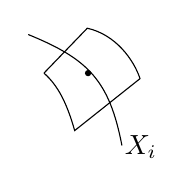
\begin{tikzpicture}[scale=1]
\draw (0.0,1.05) -- (0.55,1.62) .. controls (0.91,1.54) and (1.14,1.22) .. (1.22,0.98) -- (0.39,0.32) .. controls (0.29,0.67) and (0.18,0.89) .. (0.0,1.05);
\draw (-0.20,1.54) .. controls (0.56,1.23) and (0.83,0.96) .. (0.99,0.13);
\fill (0.56,1.05) circle (0.04);
\node at (1.23,0.11) {$X_i$};
\end{tikzpicture}
\end{adjustbox}
\end{center}

Точка $x_0\in X_i$ имеет такую окр. $U$, что

в стратификации
\begin{equation*}
U\supset U\cap X_{n-1}\supset U\cap X_{\text{\Unclear{GELFAND-P000922}{stratification-repeated-index}{$n-1$}}}\supset\ldots\supset U\cap X_i\tag{2}
\end{equation*}
[Зачёркнуто: \Incomplete{GELFAND-P000922}{cancelled-local-triviality}{Зачёркнутая строка не читается полностью; возможны начало «диффеоморфна» и конец «стратификации», средняя часть не читается.}]

во всех точках $U\cap X_i$ устроена одинаково

Рассм. циклы из [вставлено над строкой, обведено: синг.] симплексов $\sigma^q$, для к-рых
\begin{equation*}
\dim(\sigma^q\cap X_{n-i})\leq q-i
\qquad (\operatorname{Codim}X_{n-i}=2i!)\tag{3}
\end{equation*}
(как то усл., к-рое было бы, если бы было общее полож. с выд. частью)

Если справа $q$ или $q-2i$ (!), то получ. обычные когомологии.

Фактор по [над строкой зачёркнут знак: \Unclear{GELFAND-P000922}{correction-above-boundaries}{неразборчиво}]
гр. от цепей, на к-рые наложено аналог. условие.

\underline{Другое опр., гипотетически эквив. этому}
% "гипотетически" reviewed at 5x, rectangle (770,2800,1300,2900).

Делинь хотел, чтобы годилось над кон. полями.

более спец. причина: есть надежда док. связ. с $L^2$-когомологиями

($L^2$ [вставлено под строкой: -формы] при подх. к страту)
% Insertion "-формы" reviewed at 5x, rectangle (250,3040,930,3180).

\underline{А. Бейлинсон.}\quad Опред. выше можно придать лок. вид (перейти
к комплексу пучков, его когом. будут когом. Макферсона).


\SourcePage{GELFAND-P000923}{unlabelled}
% Original directly viewed at native resolution, including margins and frame boundaries.
% Text crops inspected at 3x, coordinates in original pixels:
% (140,60,2190,455), (150,455,2200,810), (215,785,2180,1330),
% (150,1290,2250,1680), (150,1660,2250,2020),
% (150,2010,2280,2490), (150,2430,2280,2910), (30,2870,1910,3370).
% Narrow readings: исп. (635,70,805,155) 6x; единств. (960,1590,1260,1710) 5x;
% F_j (380,3110,590,3250) 8x; other narrow reviews recorded in ledger.
Сейчас то же с исп. дифф. операторов

Вложим
\begin{equation*}
X\hookrightarrow \underset{\text{мн-ие [без особенностей]}}{Y}
\end{equation*}
\begin{equation*}
X_{\mathrm{reg}}=X_n-X_{n-1}\hookrightarrow X\hookrightarrow Y.
\tag{4}
\end{equation*}

На $X_n-X_{n-1}$ рассм. трив. сис. д.у., т.е.

пучок $\mathcal O_{X_{\mathrm{reg}}}$ --- пучок ф-й; он же пучок мод. над кольцом дифф. опер.

Хотим продолжить это на всё $Y$.

\underline{Пример:}

$X$ --- крест,

$Y$ --- плоскость

% The four inward arrows were inspected at 5x, original rectangle (610,805,890,1000).
\begin{center}
\begin{adjustbox}{max width=\linewidth}
\begin{tikzpicture}[scale=0.8]
\draw[->] (-1.5,0.04) -- (-0.13,0.04);
\draw[->] (1.25,-0.02) -- (0.13,-0.02);
\draw[->] (0.05,1.15) -- (0.02,0.15);
\draw[->] (-0.13,-1.0) -- (-0.06,-0.15);
\end{tikzpicture}
\end{adjustbox}
\end{center}
\SourceFigure{GELFAND-P000923}{example-cross-left-point}{Слева от внешнего конца левой горизонтальной стрелки отдельная тёмная точка; её принадлежность схеме неясна.}

продолж. ф-и, тензорно умножая на $\delta$ по трансверсали

На них действуют дифф. операторы.

(и в общ. случае так)

Вдоль $X$ должны быть регул. (и сосред. на $X$).

Рассм. пучок
\begin{equation*}
U\longrightarrow \text{все сеч. над }\bigl(\text{\Unclear{GELFAND-P000923}{sheaf-sections-domain}{$Y-X_{\mathrm{sing}}$}}\bigr)\text{ постр. пучка.}
\end{equation*}

(5)\quad (прямой образ в смысле теор. пучков при влож.
$\underline{Y-X_{\mathrm{sing}}\overset{i}{\hookrightarrow}Y}$)

(6)\quad \underline{Теор. 1.}

В этом пучке мод. есть \underline{единств. неприв. подмодуль!}

(\underline{Мораль!} (И.М.Г.) в теории особ. надо работать с дифф. операторами.)

Итак, строится модуль над кольцом дифф. опер. над $Y$.

(пучок модулей)

На $X_{\mathrm{reg}}$ рассм. пучок ф-и и прод. их $\delta$-ф-ями в трансверс. напр.

Получ. на $Y\setminus X_{\text{\Unclear{GELFAND-P000923}{overwritten-sing-index}{$\mathrm{sing}$}}}$ модуль над дифф. опер. (с голом. или алгебр. коэфф.)

\underline{Продолжаем в особенность} $X_{\mathrm{sing}}$.

Модуль стр. в 2 шага

\underline{1 шаг.} Максим. --- прямой образ пучка.

\underline{2 шаг.} Берём неприв. подмодуль (он единственен!!)

\underline{Здесь:} регулярные вдоль $X$; но без согласования!

\begin{center}
\begin{adjustbox}{max width=\linewidth}
\begin{tikzpicture}[scale=0.65]
\draw (-1,0) -- (1,0);
\draw (-0.15,-0.85) .. controls (-0.04,-0.25) and (0.09,0.38) .. (-0.03,0.8);
\fill (0,0) circle (0.08);
\end{tikzpicture}
\end{adjustbox}
\qquad (4 разных предела!)
\end{center}

[Над словом «резольвенту» зачёркнуто: \Incomplete{GELFAND-P000923}{cancelled-resolution-word}{Зачёркнутое слово не читается.}]

Рассм. резольвенту этого модуля $M$
\begin{equation*}
\ldots\longrightarrow F_1\longrightarrow F_0\longrightarrow M\longrightarrow0
\tag{7}
\end{equation*}

($F_j$ --- своб. мод. над дифф. опер.
[зачёркнут знак: \Unclear{GELFAND-P000923}{cancelled-ring-symbol}{неразборчиво}]
$\mathcal D_Y$)

и отобр. в ф-и над $Y$ (в $\mathcal O_Y$)


\SourcePage{GELFAND-P000924}{7}
% Original 2440 x 3480 directly viewed at native resolution, including margins and all frame boundaries.
% Text review at 3x, original pixel rectangles: (115,40,2260,565), (130,545,2270,1130),
% (135,1100,2290,1480), (135,1460,2290,1940), (145,1920,2350,2360),
% (145,2320,2350,2780), (145,2740,2350,3170).
% Further narrow readings: end of correspondence statement (2120,1350,2300,1460) 5x;
% marginal torsion note (1320,2135,2070,2300) 5x; filtration verb "имеет"
% (1430,2820,1940,2950) 5x; quantifier (835,2720,1030,2840) 7x.
% Corrected narrow rereading: "и неприв. факторы" (935,2810,1725,2960) 5x;
% "и" (990,2835,1110,2940) 10x; "факторы" ending (1495,2820,1645,2970) 8x.
\begin{equation*}
\bullet\longrightarrow F_1\longrightarrow F_0\longrightarrow M\longrightarrow0
\end{equation*}

Воз\Unclear{GELFAND-P000924}{complex-verb-letter}{н}. комплекс:
\begin{equation*}
\operatorname{Hom}_{\mathcal D}(F_0,\mathcal O_Y)
\longrightarrow\operatorname{Hom}_{\mathcal D}(F_1,\mathcal O_Y)
\longrightarrow\ldots\tag{8}
\end{equation*}

до $\operatorname{Codim}_Y X$ это \underline{ациклично}, а дальше Макферс. когомологии

(9)\quad \underline{Простейшие переопр. сист. д.у.} --- те, у к-рых лок. сущ. $\max$ кол-во

(10)\quad решений (привод. к системе $\dfrac{\partial u}{\partial x_1}=0,\ldots,\dfrac{\partial u}{\partial x_n}=0$) --- они
\Unclear{GELFAND-P000924}{systems-abbreviation}{цел.} опр. сист.

своих реш. --- будет лок. пост. пучок на мн-ии.

Реш. лок. --- $\mathrm{const}$.

Глобальных реш. может не быть

Аналог в общей сит.

Рассм. любую переопр. сист.

(11)\quad Если сист. имеет \underline{рег. особенности} (есть опред.), то решения ---

--- Макферс. комплекс.

[Справа, стрелка $\uparrow$ к «рег. особенности»: обобщ. пон. фуксовой сист.]

Это устанав. соотв. между этими компл. и сист. с рег. особ.

\underline{Определение} (\underline{Кашивара}) \underline{сист. с рег. особ.}

Классич. опред. (для сист. обыкн. ур-й) --- рег. особ. (Фуксова сист.):
\begin{equation*}
\frac{dx}{dt}=\frac{1}{t}A(t)x,\quad\text{где }A\text{ регул.}\tag{12}
\end{equation*}

(сист. 1-го порядка)

Пусть [зачёркнут знак: \Unclear{GELFAND-P000924}{cancelled-before-module}{неразборчиво}]
дан $\mathcal D$-модуль $M$ (связ. с переопр. сист.)

(13)\quad а) Пусть $M$ не имеет кручения, т.е. если $x\in M$, $x\ne0$,

$f\in\text{\Unclear{GELFAND-P000924}{torsion-ring}{$\mathcal D$}}$, $f\ne0$, то $fx\ne0$.

[Справа:] (нет ничего, сидящего вдоль мн-ий)

[Зачёркнуто: Тогда \Incomplete{GELFAND-P000924}{cancelled-restriction-word}{Зачёркнутое слово не читается.}
треб., чтобы суж. вдоль дост. рег. кривой

име\Incomplete{GELFAND-P000924}{cancelled-restriction-ending}{Зачёркнутый конец слова не читается.} вид (12)]

(14)\quad Тогда она прив. к сист. (10)

(15)\quad \underline{Утв.} У $M$ рег. особ. $\Longleftrightarrow$ ур., вдоль дост. рег. кривой имеют

вид (12)

\underline{Общее опр.} В $\forall$ модуле есть фильтрация

(конечная длина!) и неприв. факторы имеет вид (10) ---

--- интегр. связность.

\underline{Опр.} Каждая неприв. компон. должна иметь регул. особ.

\SourcePage{GELFAND-P000925}{unlabelled}
% Original inspected at 2440 x 3480. Coordinates below are original pixels (x0,y0,x1,y1), origin upper left.
% Reviewed at 3x: (180,2150,1150,2390), (160,2360,2410,2550), (160,2530,2260,2650),
% (260,2620,2060,3020), (160,3000,1590,3400). Further review: (2000,2390,2375,2510) 6x;
% (1200,2385,1430,2490) 6x; (300,2635,850,2745) 5x; (410,2760,1120,2945) 5x; (520,2995,730,3090) 8x.
\underline{27.10.80}\qquad \underline{\underline{Сем. Гельфанда.}}

Задачи (для первокурсников) [Подчёркнуто пунктиром.]

1. Найти все подгруппы и норм. подгруппы
\Unclear{GELFAND-P000925}{task1-group-ending}{группы / группа [окончание густо переписано]}
симметрии правильных многогранников
и симметрической группы.

2. Односвязна ли группа $SL(2,R)$? Построить её универ. накрывающую.
\begin{gather*}
\alpha\delta-\beta\gamma=1
\Longleftrightarrow \alpha_1^2-\alpha_2^2-\alpha_3^2+\alpha_4^2=1
\Longleftrightarrow \alpha_1^2+\alpha_4^2=1+\alpha_2^2+\alpha_3^2
\Longleftrightarrow \\
\Longleftrightarrow
\left(\underbrace{\frac{\alpha_1}{\sqrt{1+\alpha_2^2+\alpha_3^2}}}_{x_1}\right)^2
+
\left(\underbrace{\frac{\alpha_4}{\sqrt{1+\alpha_2^2+\alpha_3^2}}}_{x_2}\right)^2=1.
\end{gather*}
[Индексы $3$ в первом знаменателе, $4$ во втором числителе и $2$ во втором знаменателе переписаны;
\Unclear{GELFAND-P000925}{circle-index-corrections}{первоначальные знаки неразборчивы}.]
\begin{gather*}
(\alpha_1,\alpha_2,\alpha_3,\alpha_4)
\underset{\text{гомотопич. эквив.}}{\longmapsto}(x_1,x_2)\in S^1.
\end{gather*}
Точнее, имеется
\begin{gather*}
SL(2,R)\underset{\text{диффеом.}}{\cong}S^1\times R^2.
\end{gather*}
3. Как устроена универ. накр. $SL(2,R)$ как группа?

\SourcePage{GELFAND-P000926}{unlabelled}
% Original inspected at 2440 x 3480; coordinates below are original pixels, origin upper left.
% Reviewed overview crops: (100,0,2300,600) 2x; (180,575,1330,1440) 3x;
% (1290,620,2330,1270) 3x; (115,1390,2040,2425) 2x; (100,2400,2330,2780) 3x;
% (100,2760,2380,3480) 2x. Additional reviewed crops and their magnifications are in the completion note.
Пусть есть 3 прямые
\begin{center}
\begin{adjustbox}{max width=\linewidth}
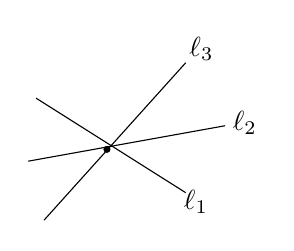
\begin{tikzpicture}[x=1cm,y=1cm]
\draw (-0.9,0.65) -- (1.0,-0.55);
\draw (-0.8,-0.9) -- (1.0,1.1);
\draw (-1.0,-0.15) -- (1.5,0.3);
\fill (0,0) circle (0.045);
\node at (1.13,-0.67) {$\ell_1$};
\node at (1.75,0.34) {$\ell_2$};
\node at (1.2,1.28) {$\ell_3$};
\end{tikzpicture}
\end{adjustbox}
\end{center}
\begin{gather*}
\text{\Unclear{GELFAND-P000926}{triple-sign-name}{$f$ / $\tau$}}(\ell_1,\ell_2,\ell_3)=
\begin{cases}
+1&\text{если $\ell_2$ внутри угла $\widehat{\ell_1\ell_3}$ (угол $<\pi$).}\\
-1&\text{в противн. случае}
\end{cases}
\end{gather*}
$(g_j,n_j)$ — элемент, $g_j\in SL(2,C)$
\Unclear{GELFAND-P000926}{group-field}{[В источнике ясно написано $C$; сохранено без исправления.]}
\begin{gather*}
(g_1,n_1)(g_2,n_2)=(g_1g_2,n_1+n_2+\tau(g_1,g_2))
\end{gather*}
[После $n_1+n_2+$ густо зачёркнуто:
\Incomplete{GELFAND-P000926}{product-cancellation}{густо зачёркнутое выражение не читается};
далее зачёркнуто $\tau(\ell_1,g_1\ell_2,g_1g_2\ell_3)$;
над ним вписано $\tau(g_1,g_2)$.]

$(\ell_1,\ell_2,\ell_3)$ можно выб. произвольно, приводя к гомолог. коциклу
\begin{gather*}
g=\begin{pmatrix}\alpha&\beta\\0&\alpha^{-1}\end{pmatrix},\qquad
\varphi(g)=\begin{cases}1,&\alpha>0\\-1,&\alpha<0\end{cases}
\\
g=\begin{pmatrix}a&b\\c&d\end{pmatrix},\qquad
\varphi(g)=\begin{cases}i,&c>0\\-i,&c<0\end{cases}
\end{gather*}
(если не прив. к треуг.)
\begin{gather*}
\psi(g,n)=e^{i\frac{\pi}{2}n}\psi(g)
\end{gather*}
\Unclear{GELFAND-P000926}{scalar-function-name}{[В этой строке знак похож на $\psi$; выше и в определении ниже написано $\varphi$.]}
Теперь надо взять
\begin{gather*}
\widetilde G=\{(g,n):\varphi(g,n)=1\}
\end{gather*}
$\widetilde G$ — это группа и она есть универ. накрывающая.

[Справа:]
(Здесь $\ell_3=\ell$ — ось $X$)
\begin{gather*}
\tau(g_1,g_2)=f(\ell,g_1\ell\,g_1g_2\ell)=\pm1
\end{gather*}
\Unclear{GELFAND-P000926}{triple-argument-divider}{[Между $g_1\ell$ и $g_1g_2\ell$ в источнике не видна запятая.]}
$\ell$ — направл. прямой

(инвар. тройки прямых; индекс тройки прямых,
[Между «тройки» и «прямых» вписано снизу и обведено: направл.]

$+1$ если $g_1\ell$ между $\ell$ и $g_1g_2\ell$

\underline{Эта гр. несвязна} — есть 4 куска;
тогда надо взять связн. комп.

4. (Кириллов). Описать все локально проективные структуры на $R$

(покр. картами, переход — дробно-лин. преобр.)

атласы эквив., если переход — др.-лин. преобр.

\underline{ответ}: есть счетное число лок. проект. структур

\underline{1 пример.} $R$ и пар. $t$

\underline{2 пример:}
\begin{center}
\begin{adjustbox}{max width=\linewidth}
\begin{tikzpicture}[x=1cm,y=1cm]
\draw[<->] (0,0) -- (2.1,0);
\draw (1,-0.08) -- (1,0.08);
\node at (1,0.3) {$t$};
\node at (1,-0.3) {$0$};
\draw[<->] (3,0) -- (4.8,0);
\draw (3.9,-0.08) -- (3.9,0.08);
\node at (3.9,0.3) {$s$};
\node at (3.9,-0.3) {$0$};
\node[anchor=west] at (5.3,0) {— настоящие};
\draw[<->] (1.5,-1) -- (3.9,-1);
\draw (2.65,-1.09) -- (2.65,-0.91);
\node at (2.65,-1.35) {$x$};
\end{tikzpicture}
\end{adjustbox}
\end{center}
\underline{Сост.:} $tx=-1,\quad xs=-1$

Кончилась одна — пер. к другой и т.д.

2-я не эквив. 1-й.

2-листное накр. на проект. прямую имеет лок. проект. структуру.

Накр. проект. прямой — ее проект. преобр. будут — обр. универ. накрытия.

\underline{Проф. Гаво} (\underline{из Парижа})\qquad \underline{3 возм. темы.}

[Над «из Парижа», со стрелкой к этой помете: \underline{Univ. Paris VI}.]

1. Констр. оболочек голоморфности

2. Констр. мер на нек-рых $\infty$-мерн. однор. мн-вах

3. Теория рассеяния и функц. интегралы.

[Справа:]
\underline{Гаво} — ученик Маллевена, к-рый сейчас
заним. стохастической дифф. геометрией.

\underline{1. О конструкциях оболочек голоморфности.}

Рассм. $C^2$ и попробуем постр. обол. голом. комп. 2-мерной пов. (в $C^2$).

\underline{Зад.} Найти такую
[зачёркнуто: \Incomplete{GELFAND-P000926}{levi-cancellation}{густо зачёркнутое слово не читается}]
Леви-плоскую гиперпов. $M$, такую что
\begin{gather*}
\partial M=S^2
\end{gather*}
(форма Леви на ней должна быть $=0$)

Леви плоские обл. рассл. на компл. линии

(На торе эту зад. решить нельзя)

\SourceFigure{GELFAND-P000926}{levi-foliation}{Справа внизу овал с несколькими приблизительно вертикальными дугами внутри, надписью $M_3$ в середине и тёмной точкой на левом краю. Слева подпись $(\partial M)_2$ со стрелкой к верхней левой части овала. На верхнем краю имеется небольшой тёмный штрих, направление которого не устанавливается. Подпись под овалом: «покрытие дисками (слоение)».}

\SourcePage{GELFAND-P000927}{11}
% Original inspected at 2440 x 3480; coordinates below are original pixels, origin upper left.
% Reviewed overview crops: (200,0,2430,500) 2x; (180,480,1520,1040) 3x;
% (150,1020,2280,1760) 2x; (300,1750,2270,2300) 2x;
% (150,2240,2350,2920) 2x; (100,2880,2360,3480) 2x.
% Further reviewed crops and their magnifications are recorded in the completion note.
Есть особ. точки слоения $\Rightarrow$ индекс
\Unclear{GELFAND-P000927}{top-index-abbreviation}{вырожд. / вырож.}
зад. Римана $=0$ $\Rightarrow$ она решается
(Бишоп — возник. син. интегро-дифф. ур-е)

\underline{2–3}

$M$ — мн-ие, $G$ — комп. гр. Ли, $g$ — алг. Ли

$\Lambda^1(M,g)$ — 1-формы на $M$ со знач. в $g$.
[У $\Lambda$ густо переписан и зачёркнут нижний индекс:
\Unclear{GELFAND-P000927}{forms-cancelled-index}{$2$?}.]

[На правом поле, отделено вертикальной чертой:]
хотим рассмотреть Янга-Миллса
\begin{gather*}
(1)\qquad e^{-\int_M\operatorname{Tr}(\Omega\Omega)}D(\omega)
\end{gather*}
[Стрелка снизу к $\Omega$: кривизна $\omega$; линия от $\omega$ в $D(\omega)$ к подписи: связность.]

(Формальный фейнман. интеграл)

\underline{Группа:}
$g\in C(M,G)$ (калибр.)
\begin{gather*}
(2)\qquad g\cdot\omega=g^{-1}dg+g^{-1}\omega g
\end{gather*}
[После второго $g^{-1}$ зачёркнуто:
\Incomplete{GELFAND-P000927}{gauge-cancellation}{густо зачёркнутое выражение не читается}.]

Цель — построить инвар. меру отн. калибр.
[зачёркнуто: \Unclear{GELFAND-P000927}{group-word-cancellation}{гр.?}]
группы.

(проще, чем на факторпр-ве)

Надо интегр. по мн-ву траекторий в $\Lambda^1$.
\begin{gather*}
(3)\qquad e^{-\int_0^t dt\int_M\operatorname{Tr}(\Omega_t\Omega_t)\,dx}D(\omega_t)
\end{gather*}
Будем построим семейство мер, «приближ.» к равнов. мере.
\Unclear{GELFAND-P000927}{measure-family-verb}{[Сочетание «Будем построим» сохранено по видимым буквам.]}

\begin{center}
\begin{adjustbox}{max width=\linewidth}
\begin{tikzpicture}[x=1cm,y=1cm]
\draw (0.55,-1) .. controls (0.02,-0.45) and (0.03,0.62) .. (0.55,1);
\draw (1.2,-1) .. controls (0.8,-0.3) and (0.73,0.55) .. (1.2,1);
\draw (1.85,-1) .. controls (1.46,-0.3) and (1.42,0.55) .. (1.85,1);
\draw (2.5,-1) .. controls (2.17,-0.3) and (2.11,0.55) .. (2.5,1);
\fill (0.16,-0.05) circle (0.04);
\node[anchor=east] at (0,-0.05) {$\Pi$};
\draw[thick] (0.16,-0.05) -- (2.8,-0.05);
\draw (0.16,-0.05) .. controls (1.05,0.5) and (1.65,0.23) .. (2.85,0.67);
\draw (1.4,0.75) -- (3.25,1.02);
\node[anchor=west] at (3.3,1.02) {орбиты калибр. гр.};
\draw (2.6,-0.05) -- (3.2,-0.45);
\node[anchor=west] at (3.3,-0.45) {трансверс. сеч.};
\end{tikzpicture}
\end{adjustbox}
\end{center}

\underline{Сначала} — типа винер. мера на путях.

Нужно что-то вроде эллипт. оператора в пр-ве связностей; инвар. отн.
калибр. группы.
\begin{gather*}
\Pi\to d_\Pi\text{ — ковар. диффер.,}\qquad
\Box_\Pi=d_\Pi^*d_\Pi+d_\Pi d_\Pi^*
\\
(4)\qquad e^{-\tau\Box_\Pi}(x,y)=p_\tau^{(\Pi)}(x,y)
\text{ — \underline{теплов.} функц.}
\\
(5)\qquad L\varphi(\Pi)=\iint_{M\times M}e^{-\tau\Box_\Pi}(x,y)
\frac{\delta^2\varphi}{\delta\Pi(x)\delta\Pi(y)}\,dx\,dy
\end{gather*}
[Зачёркнуто: \Incomplete{GELFAND-P000927}{fixed-tau-cancellation}{знак или короткое слово под зачёркиванием не читается}.]
\underline{$\tau$ фиксирован.}

Нельзя раб. в соб. пр-вах.
\begin{gather*}
(6)\qquad\Lambda^1_{k,\alpha}(M,g),\quad 0<\alpha<1,
\end{gather*}
— какое-то пр-во (гёльдеровские)

$k$-я пр. им. гёльд. на $\alpha$.

Нужно:
\begin{gather*}
(7)\qquad
\left\|e^{-\tau\Box_\Pi}-e^{-\tau\Box_{\Pi'}}\right\|_{HS}
\le C\|\Pi-\Pi'\|
\end{gather*}
[Под $HS$: Гильб.-Шмидта.]

\SourcePage{GELFAND-P000928}{unlabelled}
% Original inspected at 2440 x 3480. Original-pixel crop coordinates, origin upper left.
% Reviewed at 3x: (60,70,1650,310), (180,280,2250,470), (60,465,1140,745), (90,720,1240,990),
% (120,950,1680,1140), (140,1100,1620,1310), (290,1300,1510,1570), (155,1570,1420,1800),
% (320,1780,2110,2100). Further review: (1220,315,1620,412) 6x; (620,440,940,550) 8x;
% (385,675,625,761) 8x; (870,1325,1170,1418) 6x; (900,1900,1120,2030) 8x;
% (1350,1125,1580,1240) 8x; (465,1430,580,1545) 10x; (775,1600,930,1740) 8x; (820,200,1045,303) 8x.
% Final noun reviewed at (710,1760,1020,1875) 6x, independently at (815,1790,980,1880) 10x.
Получается
\begin{gather*}
(8)\qquad
\left\|e^{-\tau\Box_{\Pi}}-e^{-\tau\Box_{\Pi'}}\right\|_{HS(L^2,L^2)}
<C\|\Pi-\Pi'\|_{k,\alpha}.
\end{gather*}
Технич. мом.: броуновское движ. зависит от пр-ва,
$e^{-\tau\Box_{\Pi}}$ возвращает обратно:
\begin{gather*}
(9)\qquad d\Pi_t=e^{-\tau\Box_{\tau}}\underbrace{d\beta_t}_{\text{белый шум}}.
\end{gather*}
\Unclear{GELFAND-P000928}{equation09-index}{[Индекс у $\Box$ имеет вид $\tau$; возможно $t$ или $\Pi$.]}

[Зачёркнуто: Интересно.]
\begin{gather*}
(10)\qquad \left(\frac12\Delta-V\right)\Psi=\frac{\partial}{\partial t}\Psi,\\
(11)\qquad \Psi_t(x)=E_x\left(\exp\left(-\int_0^t V(b_\omega(s))\,ds\right)\Psi_0(b_\omega(t))\right).
\end{gather*}
В частности,
\begin{gather*}
(12)\qquad \pm\lambda_1=\lim_{t\to\infty}
\frac{\log E_x\bigl(\exp\bigl(-\int_0^t V(b_\omega(s))\,ds\bigr)}{t}.
\end{gather*}
\Unclear{GELFAND-P000928}{equation12-parentheses}{[В числителе после $ds$ видна одна закрывающая скобка.]}

(Интересно, напр., когда есть отриц. уровни)

Пусть
\begin{gather*}
(13)\qquad |\Delta^{-1}V|\le C<1.
\end{gather*}
[Знак перед $^{-1}$ переписан:
\Unclear{GELFAND-P000928}{equation13-operator}{$\Delta$ или $\Box$; первоначальное чтение не установлено}.]
Тогда
\begin{gather*}
(14)\qquad E_x\left(\exp\left(-\int_0^\infty V(b_\omega(s))\,ds\right)\right)
\le\frac{1}{1-C}.
\end{gather*}
[Буква в аргументе $V$ густо переписана:
\Unclear{GELFAND-P000928}{equation14-path}{$b_\omega$ или $B_\omega$}.]
$\Rightarrow$ оценив. соб. \Unclear{GELFAND-P000928}{eigenvalue-word}{значение}.

$V\longmapsto\varepsilon V$\quad
\Unclear{GELFAND-P000928}{last-line-abbreviation}{пол. / пот.}, взяли $\varepsilon$ мало
$\Rightarrow$ что-то оценивается.


\SourcePage{GELFAND-P000929}{unlabelled}
\underline{\underline{3/$\overline{\underline{\mathrm{XI}}}$-80 г.}}\qquad \underline{Сем.} \underline{Гельфанда.}

\underline{И.М.Г.}\qquad \underline{История теории представлений}

1. Дедекинд — характеры конечн. коммут. групп (для $L$-ф-ий)

2. Фробениус — матрицы и следы для некоммут. групп

3. Хаар (рано умер)

(*)4. фон Нейман — теория $C^*$-алгебр для предст. некоммут. групп

(**)5. Гельфанд и Наймарк — о предст. гр. Лоренца

\underline{Идеология} (*): всё устроено теоретико-множественно

\hspace{2em}(**). —$\Vert$— гладко и просто

Совр. анализ: некоммут. дифф. геометрия и интегр. геометрия.

{\small Надо учит. \Unclear{GELFAND-P000929}{inserted-structure}{алгебр.} структуру.}

Групп. алгебра для алг. Ли — \underline{оберт. алгебра.}

но: их всё равно много (нет теор. \Unclear{GELFAND-P000929}{wedderburn-name}{Веддербарна})

\underline{Гельфанд, Кириллов.} тело отн. оберт. алг. $\cong$ тело отн. кольца дифф. операторов

Это не доделано. (Недостаточно опер. с полин. коэффициентами, частично это
понято в раб. [Зачёркнуто: \Unclear{GELFAND-P000929}{cancelled-before-novikov}{неразборчиво}] Новикова, Кричевера, Шабата и т.п.)

\underline{Бернштейн, С. Гельфанд, И.М. Гельфанд}\qquad в проект. пр-ве.

Надо раб. с пучками.

Сейчас уже надо \Unclear{GELFAND-P000929}{last-line-verb}{прослушивать} не теорию предст., а то, для чего она делается.

\SourcePage{GELFAND-P000930}{16}
\underline{А. Бейлинсон}

$X$ — алгебр. мн-зие над $\mathbb{C}$

Самые простые — аффинные.

Они однозн. опред. кольцом ф-й на них.

\underline{Коммут. кольцо} $=$ [Зачёркнуто: \Unclear{GELFAND-P000930}{cancelled-affine-word}{алгеб.}] \underline{аффинное алг. мн-зие.}

\underline{Модули над ним} $=$ \underline{квазикогер. пучки}

$X=\mathrm{Spec}\,A$, $M$ — $A$-модуль (всегда топ. Зарисского)

Базис откр. мн-в: $X_f=\{x:f(x)\ne 0\}$.

$O(X_f)=A_f$ — локализация $A$ по $f$.

\begin{equation*}
\mathcal{M}(X_f)=M_f=M\otimes_A A_f.
\end{equation*}

Получ. пучок на $\mathrm{Spec}\,A$. Так получ. класс квазикогер. пучков на $X$.

\underline{Будет некоммут. аналог локализации} (переход от мод. к пучку).

(1) \underline{Кольца}: \underline{универс. оберт. алг. полупр. алг. Ли и их факторы.}

$X$ — алг. мн. — наз. $\mathcal{D}$-\underline{аффинным}, если оно облад. св-вом

($\mathcal{D}_X$ — пучок колец дифф. опер. на $X$)

{\small [Слева приписано: Счит., что]} $X$ — гладкое;

$\mathcal{M}$ — пучок модулей над $\mathcal{D}_X$; $O_X\subset\mathcal{D}_X$ (подпучок; дифф. оп. 0-го пор.)

$\mathcal{M}$ наз. \underline{квазикогерентным}, если он квазиког. как пучок $O_X$-модулей.

(\underline{Пример}: сам $\mathcal{D}_X$ квазикогерентен).

$X$ — алгебр. мн-зие, $O_X$ — пучок ф-й на нём; пучок $\mathcal{M}$ $O_X$-модулей на $X$
наз. \underline{квазикогерентным}, если он облад. след. св-вом:

$\forall$ аффинного мн-ва $U$ и его афф. подмн-ва $U'\subset U$ должно быть:

\begin{equation*}
(2)\qquad \mathcal{M}(U')=\mathcal{M}(U)\otimes_{O(U)}O(U').
\end{equation*}

(ясно, что правая часть (2) отобр. в левую, треб., чтобы это
было изоморфизмом)

(3) \underline{Утверждение}. $X$ аффинно $\Longleftrightarrow$ $\forall$ квазикогер. $\mathcal{M}$

(4) $\underset{i>0}{H^i(X,\mathcal{M})=0}$ и $\mathcal{M}$ порожд. над \Unclear{GELFAND-P000930}{generation-ring}{$O(X)$} глоб. сечениями, т.е.

\begin{equation*}
(5)\qquad H^0(X,\mathcal{M})\otimes O_X
\underset{\text{\underline{эпиморфизм}}}{\longrightarrow}\mathcal{M}
\end{equation*}

(Не совсем трив. теорема — Серр, Гротендик — см. раб. Серра о ког. пучках)

\SourcePage{GELFAND-P000931}{unlabelled}
(6). \underline{Определение}. $X$ наз. $\mathcal{D}$-\underline{аффинным}, если $\forall$ квазикогер. пучка
$\mathcal{D}$-модулей $\mathcal{M}$ вып. условия (4), (5), т.е.

[Зачёркнуто: \Unclear{GELFAND-P000931}{cancelled-before-7}{неразборчивая прежняя метка}]
\begin{equation*}
(7)\qquad H^i(X,\mathcal{M})=0,\ i>0
\end{equation*}
\begin{equation*}
(8)\qquad H^0(X,\mathcal{M})\otimes\mathcal{D}_X\longrightarrow\mathcal{M}\longrightarrow 0
\end{equation*}

(9) \underline{Примеры}.

1. $\forall$ афф. мн-зие — $\mathcal{D}$-аффинно.

2. $\forall$ проект. пр-во $\mathbb{P}^N$ — $\mathcal{D}$-аффинно.

(частн. случай теор., о к-рой будет идти речь)

3. Эллипт. кривая — не $\mathcal{D}$-аффинна

(10) \underline{Следствие} $\mathcal{D}$-\underline{аффинности}

Пусть $X$ — мн-зие, $\mathcal{L}$ — пучок $O$-модулей, рассмотрим

(11) $\mathcal{D}_X\otimes_{O_X}\mathcal{L}$ — квазикогер. пучок $\mathcal{D}_X$-модулей

{\small [Над строкой зачёркнуто: \Unclear{GELFAND-P000931}{cancelled-above-12}{неразборчиво}]}

(12) $X$ — $\mathcal{D}$-афф. $\Rightarrow$ когомологии пучка (11) равны 0 и он порожд.
глоб. сеч. (т.е. вып. (7) и (8)), даже если сам $\mathcal{L}$
был плохой

(13) (Например, \Unclear{GELFAND-P000931}{twist-index-13}{$O(-i)$} на $\mathbb{P}^N$, он не имеет сечений и имеет
высшие когомологии)

{\small Например.}

(14) $\mathcal{D}_X\otimes_{O_X}$ \Unclear{GELFAND-P000931}{twist-index-14}{$O(-i)$} на $\mathbb{P}^N$ порожд. глоб. сечениями

(докладчик не знает прямого док-ва)

К сожалению, нет хорошей записи $\mathcal{D}_X$, т.к. дифф. опер. глобально не
записывается в виде суммы однородных.

(14) — некий лок. свободный $\mathcal{D}_X$-модуль

$\mathcal{D}_X$ в (11) рассматривается как правый пучок $O_X$-модулей

Если рассмотреть

\begin{equation*}
(15)\qquad O(-i)\otimes_{O_X}\mathcal{D}_X,
\end{equation*}

то это будет уже не так; он не порожд. глоб. сеч. и
высш. когом. $\ne 0$ ($O(-i)$ — его прямое слагаемое)

[Зачёркнуто: Эллипт. кривая]\qquad \underline{Об эллипт. кривой}

(16) Пусть на $\mathcal{D}_X$ есть инволюция, тож. на $O_X$, и \Unclear{GELFAND-P000931}{involution-product}{$\underline{ab}\overset{*}{\mapsto}\underline{ba}$};
тогда (14) и (15) были бы изоморфны и мн-зие не было бы
$\mathcal{D}$-афф. Но на элл. кривой есть \underline{инволюция} — взятие формально
сопр. оператора \Unclear{GELFAND-P000931}{formal-adjoint-sign}{$f\frac{\partial}{\partial x}\mapsto\frac{\partial}{\partial x}f$}
\Unclear{GELFAND-P000931}{last-parenthesis}{(если сопр. — всё хор. с пост. коэфф.)}

\SourcePage{GELFAND-P000932}{17}
От $\mathcal D_X$ отщепляется кольцо ф-й $\Rightarrow$ (25) не ациклично

(17) \underline{Утверждение.} $X$ — \underline{$\mathcal D$-аффинно}, \underline{тогда}
\Unclear{GELFAND-P000932}{line17-cancel}{Зачёркнутое слово не разобрано.}
\underline{функтор сечений} $\Gamma$
\begin{equation*}
\mathcal D_X\text{-mod}\overset{\Gamma}{\longrightarrow}
\Gamma(\mathcal D_X)\text{-mod},
\tag{18}
\end{equation*}
\underline{является эквивалентностью категорий.}

(Докладчик \Unclear{GELFAND-P000932}{note-after-speaker}{Малый замазанный знак после слова «Докладчик».}
не знает, вытекает ли отсюда $\mathcal D$-аффинность; в коммут. случае это так)

\begin{equation*}
D_X\underset{\mathrm{def}}{=}\Gamma(\mathcal D_X)
\tag{19}
\end{equation*}

\Unclear{GELFAND-P000932}{before20-cancel}{Зачёркнуто: возможно, «Теорема».}

(20) \Unclear{GELFAND-P000932}{condition20-scope}{Достат. условие не $\mathcal D$-аффинности} —
\Unclear{GELFAND-P000932}{line20-cancel}{Зачёркнутая запись перед $ch_1$ не разобрана.}
$ch_1$ (пучка форм. макс. степени) $=0$

\begin{equation*}
\bigl(\Leftrightarrow ch_1(\text{касат. рассл.})=0\bigr)
\tag{21}
\end{equation*}

\begin{equation*}
(20)\Leftrightarrow(21)\Leftrightarrow\text{сущ. инволюции.}
\tag{22}
\end{equation*}

(Дифф. опер. с перест. $x$ и $\frac{\partial}{\partial x}$ —
дифф. опер. на формах max степ.)

\textit{[Межстрочная вставка:]}
Изом. обр. пучков $\Leftrightarrow ch_1$ совпадают
\Unclear{GELFAND-P000932}{insert-circled-word}{Под $ch_1$ обведено: «лин.» или «алг.».}

(23) \underline{Теорема.} $G$ — \underline{полупр. группа} Ли,
$B$ — \underline{борелевская подгр.},
\underline{рассм.} $X=G/B$ — ("пр-во флагов") \underline{Тогда}
\textit{[Зачёркнуто:]} $X$ — $\mathcal D$-аффинно и

1. $X$ — $\mathcal D$-аффинно

2. $D_X=U(\mathfrak g)/U(\mathfrak g)I_0$;

\begin{quote}
\textit{[На правом поле; слева квадратная скобка:]}

(*) \Unclear{GELFAND-P000932}{example-cancel}{Зачёркнутая запись в скобках не разобрана.}

\underline{Пример:} $G=SL(2,\mathbb C)$,

$B$ — треуг.

$G/B=\mathbb P^1$

какие дифф. опер. на $\mathbb P^1$?
\end{quote}

где
\begin{equation*}
\begin{adjustbox}{max width=\linewidth}
\begin{tikzcd}[column sep=small,row sep=small]
I_0=\ker\{ & Z(\mathfrak g)\arrow[r] & \mathbb C\} \\
& U(\mathfrak g)\arrow[u,phantom,"\cap" description]\arrow[ur]
& \text{— станд. единств. одном. характер}
\end{tikzcd}
\end{adjustbox}
\tag{24}
\end{equation*}

$I_0$ — операторы Лапласа без своб. члена

\Unclear{GELFAND-P000932}{before25-cancel}{Зачёркнуто: возможно, «Утверждение».}
\underline{Предложение.}

(25) \underline{$D_X$-модули} $\Leftrightarrow$ \underline{представления} $\mathfrak g$,
\underline{на к-рых трив. действует} $I_0$.

($Z(\mathfrak g)$ должно действ. как на трив. 1-мерном представлении)

\underline{Пример (*).}

(26) На $\mathbb P^1$ есть \textit{[вписано и обведено:]} дифф. опер.
\begin{equation*}
\begin{adjustbox}{max width=\linewidth}
\begin{tikzpicture}
\node (operators) {$\frac{d}{dx};\quad x\frac{d}{dx}\quad\text{и}\quad x^2\frac{d}{dx}$};
\draw (operators.south west) -- ++(0,-0.12) -| (operators.south east);
\end{tikzpicture}
\end{adjustbox}
\end{equation*}
Берутся полиномы от них — это обёрт. алгебра.

Есть единств. опер., перест. со всеми. (Шварцман?)

\underline{Мораль:} теория представлений сводится к теории $\mathcal D_X$-модулей.

\underline{Улучшение по ср. с известным:} можно локализовать!!

\SourcePage{GELFAND-P000933}{unlabelled}
\Unclear{GELFAND-P000933}{above-date-marks}{Над датой отдельные штрихи; буквенная запись не читается.}

\underline{\underline{10.11.80 г.}}\qquad \underline{Сем. Гельфанда.}

\underline{И.М.Г.}\qquad \underline{\underline{Числа Кэли.}}

\Unclear{GELFAND-P000933}{formula1-overwritten-number}{У номера (1) слева жирный переписанный или зачёркнутый штрих; первоначальный знак не установлен.}
\begin{equation*}
\left|\sum_{j=1}^{8}x_j e_j\right|
=\sqrt{\sum_{1}^{\Unclear{GELFAND-P000933}{right-sum-upper-limit}{2\text{ или }8}}x_j^2}
\tag{1}
\end{equation*}

В числах Кэли:
\begin{equation*}
|ab|=|a||b|
\tag{2}
\end{equation*}

Как док., что нет $>8$ измер.?

Получ. задача из теории. предст. благодаря (2) и явная конструкция.

\underline{Вопрос:} \underline{может быть, бывает в $\infty$-мерном пр-ве?} (с усл. (2))

Гиндикин утв., что бывает. Надо повторить док-во того,
что в конечномерном случае ничего не бывает, кроме $\mathbb R,\mathbb C,\mathbb H$ и Кэли.

Проективные геометрии (плоскости).

Ввод. координаты, ассоциативность $\Leftrightarrow$ дезарговость

Проект. плоскость Кэли — простейшая \underline{недезаргова}

Интересно изучить диффер. и лок. однородные проект. плоскости.

— Зад. классиф. алгебр Ли — слишком частная
(надо, чтобы не было обрывков
$G_2,E_6,E_7,E_8$ и т.п.

\underline{\underline{Бейлинсон.}}\qquad
\underline{О локализации представлений.}

$X$ — алг. мн-ие (над $\mathbb C$),

$\mathcal A$ — квазикогерентный $\mathcal O_X$-модуль

\textit{[Под $\mathcal A$ вертикальный штрих к следующей строке:]}
пучок колец, содержащий $\mathcal O_X$.
(включение $\mathcal O_X\subset\mathcal A$ \textit{[вписано снизу:]} задано)

(Напр., $\mathcal A$ — пучок дифф. операторов)

\underline{$\mathcal A$-mod} — \underline{категория пучков левых} $\mathcal A$-\underline{мод.},
\underline{явл. квазикогер}
$\mathcal O_X$-\underline{модулями}

\SourcePage{GELFAND-P000934}{20}
(В прошлый раз было $\mathcal A$ — дифф. опер.)

$A=\Gamma(\mathcal A)$,\quad $A$-mod — катег. $A$-модулей (левых).

Есть 2 сопр. функтора.
\begin{equation*}
\begin{adjustbox}{max width=\linewidth}
\begin{tikzcd}[column sep=large]
\mathcal A\text{-mod}\arrow[r,"\Gamma"]
& A\text{-mod}\arrow[l,bend left=30,"\Delta"]
\end{tikzcd}
\end{adjustbox}
\tag{1}
\end{equation*}

\begin{equation*}
\Delta(M)=\mathcal A\otimes_A M,
\tag{2}
\end{equation*}
$M$ рассм. как пост. пучок \Unclear{GELFAND-P000934}{constant-module-notation}{$\mathcal A$-мод.} над $X$
(слой $=M$ над каждой точкой) и отобр. тривиальны.

Легко видеть, что они сопряжены.

(3) \underline{Опрд.-лемма.}
\Unclear{GELFAND-P000934}{definition-cancel}{После заголовка зачёркнутый знак, возможно «а)».}

\underline{Мн-ие $X$ наз. $\mathcal A$-аффинным, если вып. одно из 2-х эквив. условий}

а) $\forall\mathcal M\in\mathcal A$-mod,
$H^i(X,\mathcal M)=0$, $i>0$ и
$H^0(X,\mathcal M)\ne0$ при $\mathcal M\ne0$.

б) \underline{Функторы $\Gamma$ и $\Delta$ являются взаимно-обратными эквивалентностями категорий.}

(На самом деле а) эквив. тому, что было в прошлый раз,
меняем модули).

а) трудно проверить, б) проще использовать.

\underline{Док-во эквивалентности а) и б).}

\underline{а) $\Rightarrow$ б).}
\begin{equation*}
\Gamma(\mathcal M)=
\operatorname{Hom}_{\mathcal A\text{-mod}}(\mathcal A,\mathcal M)
\tag{4}
\end{equation*}

(образ $1$ — сечение $\mathcal M$).

(5) а) $\Rightarrow$ $\mathcal A$ — проективная образующая в катег. $\mathcal A$-mod.

(6) (такой объект, что i) $\operatorname{Hom}(\mathcal A,\mathcal M)$ —
\underline{точный} функтор

(7) ii) $\forall$ ненулев. объекта $\mathcal M$;
$\operatorname{Hom}(\mathcal A,\mathcal M)\ne0$)

(из ацикличности вытекает i), а из 2-го условия ii))

(точный функтор — перев. точные посл. в точные)

i) — св-во проективности

ii) — образующая

(кстати, ii) $\Rightarrow$ можем отобразить $\mathcal A$ в фактор
$\mathcal M/\operatorname{Im}t$ и т.д.)

(8) iii) $\Gamma$ перев. прямые суммы в прямые суммы.
\begin{equation*}
\Gamma(\oplus\mathcal M_i)=\oplus\Gamma(\mathcal M_i)
\end{equation*}

\SourcePage{GELFAND-P000935}{unlabelled}
(св-во любых квазиког. пучков)

\underline{Общекатег. факт}

(9) \underline{Лемма.} Пусть зад. $\forall$ категория $C$ (абелева), $X\in C$,

[Над строкой, с выноской к «(абелева)»: «с прямыми суммами в $\forall$ кол-ве.»]

$X$ — Проект. образующая со св-вом (8):

(10) $\operatorname{Hom}_C(X,\cdot)$ коммут. с прямыми суммами.

(11) [Зачёркнуто: «Тогда».]
$\operatorname{Hom}_C(X,\cdot):C\longrightarrow \operatorname{End}_C X\text{-}\mathrm{mod}$

Тогда этот функтор — \underline{эквивал. категорий}.

Из леммы все вытекает, если применить её к случаю, когда

\begin{equation*}
(12)\qquad C=\mathcal{A}\text{-}\mathrm{mod},\quad X=\mathcal{A},\quad \operatorname{End}_C X=A
\end{equation*}

Обр. импликация $\underline{\text{б)}\Rightarrow\text{а)}}$ \underline{из} резольвенты Чеха.

$\mathcal{D}$-аффинное мн-зие, — мн-зие, $\mathcal{A}$-афф. при $\mathcal{A}=\mathcal{D}_X$.

(13) \underline{Теор.} $\mathbb{P}^{N}$ — $\mathcal{D}$-\underline{аффинно}.

\Unclear{GELFAND-P000935}{theorem-heading}{Следующая} теорема:

$G$ — редуктивная группа.

$X=G/B$ — пр-во флагов

($B$ — борелевская подгруппа)

(14) $x\in X\Rightarrow B_x$ — соотв. борелевская подгруппа

[Под $B_x$: «(стац.)».]

$G$ — действ. на $X\Rightarrow\mathfrak{g}$ действ. на $X$.

\begin{equation*}
(15)\qquad \mathfrak{g}\longrightarrow \operatorname{Vect}X
\end{equation*}

отсюда.

\begin{equation*}
(16)\qquad U(\mathfrak{g})\longrightarrow D_X=\Gamma(\mathcal{D}_X).
\end{equation*}

\begin{equation*}
(17)\qquad \underset{\substack{\downarrow\\\text{центр}}}{Z(\mathfrak{g})}\subset U(\mathfrak{g})
\end{equation*}

$I$ — аннулятор единичного предст. \Unclear{GELFAND-P000935}{annihilator-final-symbol}{$\mathfrak{g}$ или $\xi$}

(max идеал в центре)

\begin{equation*}
(18)\qquad J=I\cdot U(\mathfrak{g}).
\end{equation*}

(19) \underline{Теорема.} а) $X$ — $\mathcal{D}$-\underline{аффинно}.

б) \underline{при} \underline{морфизме} (16) \underline{получается} \underline{изоморфизм}

\begin{equation*}
(20)\qquad U(\mathfrak{g})/J\overset{\sim}{\Rightarrow}D_X
\end{equation*}

(21) Отсюда, эквив. категорий 1) $\mathcal{D}$-пучков на $X$ и 2) представлений
алг. Ли $\mathfrak{g}$ с един. инфинитезим. характером.

\SourcePage{GELFAND-P000936}{21}
[Зачёркнуто: \Unclear{GELFAND-P000936}{cancelled-heading}{неразборчивый заголовок}.]
\underline{Вступление.}

$X,Y$ — \Unclear{GELFAND-P000936}{opening-word}{два или оба} гладких алгебр. мн-зия.

$X\overset{f}{\longrightarrow}Y$ отображение.

Тогда имеются категории $\mathcal{D}_X\text{-}\mathrm{mod}$ и $\mathcal{D}_Y\text{-}\mathrm{mod}$

Есть 2 функтора в пучках $f^*$ и $f_*$.

Но в дифф. опер. нет никакого соответств. морфизма.

Но функторы (естеств.) есть; они опр. на уровне производной категории

(на самом деле есть \underline{4 функтора})

(22) $f^{\circ}$ — обр. образ в кат. \underline{\underline{пучков}}.

\begin{equation*}
(23)\qquad \mathcal{O}_X\otimes_{f^{\circ}\mathcal{O}_Y}f^{\circ}(\mathcal{D}_Y)
\end{equation*}

\begin{equation*}
(24)\qquad \mathcal{D}_{X\to Y}\underset{\mathrm{def}}{=}\mathcal{O}_X\otimes_{f^{\bullet}\mathcal{O}_Y}f^{\bullet}\mathcal{D}_Y
\end{equation*}

\begin{equation*}
(25)\qquad \mathcal{D}_{X\to Y}\text{ — }
\left\{\begin{array}{l}
\text{лев. }\mathcal{D}_X\text{-модуль}\\
\text{прав. }f^{\circ}\mathcal{D}_Y\text{-модуль}
\end{array}\right.
\end{equation*}

лев. $\mathcal{D}_X$ по правилу Лейбница; ост. для вект. полей на $X$:

$v\in\operatorname{Vect}X$;

\begin{equation*}
(df)(v)\in\Gamma(f^*T_Y)
\end{equation*}

\Unclear{GELFAND-P000936}{final-left-mark}{жирная наклонная отметка; возможно «!»}
$(df)(v)$ действует на $\underline{\underline{f^{\bullet}\mathcal{D}_Y}}$.

\SourcePage{GELFAND-P000937}{unlabelled}
\underline{\underline{17.11.80 г.}}\qquad \underline{Сем. Гельфанда}

\underline{И.М.Г.}\quad \underline{задачи.}

1.
\begin{equation*}
f(x)=\left\{\begin{array}{ll}
1/q,&x=p/q\text{ — несокр.}\\
0,&x\text{ — иррац.}
\end{array}\right.
\end{equation*}

Где она непрерывна?

где она дифференц.?

\begin{equation*}
f(x)=\left\{\begin{array}{ll}
1/q^{\alpha},&x=p/q\text{ — несокр.}\\
0,&x\text{ — иррац.}
\end{array}\right.
\end{equation*}

Что можно сказать о дифф.?

2. $f(x)=\lim\limits_{n\to\infty}\lim\limits_{m\to\infty}(\cos^{2m}2\pi n!x)$ — ф-я Дирихле.

3. Можно ли построить ф-ю Дирихле с одним знаком предела?

(из непр. ф-й)

[Справа вверху:]

4. Вычислить приближенно $\displaystyle\int_{-\infty}^{\infty}e^{-x^2}\cos1000x\,dx$

То же с $e^{-x^4}$ или $e^{-x^6}$

\underline{А. Бейлинсон.}

$X\overset{f}{\longrightarrow}Y$,\quad $X,Y$ — мн-зия.

$\mathcal{D}_X\text{-}\mathrm{mod},\ \mathcal{D}_Y\text{-}\mathrm{mod}$ — категории квазиког. пучков $\mathcal{D}_X\text{-}\mathrm{mod}$ и $\mathcal{D}_Y\text{-}\mathrm{mod}$ на $X$ и $Y$

\begin{equation*}
\mathcal{D}_X\text{-}\mathrm{mod}\quad\substack{\longrightarrow\\\longleftarrow}\quad\mathcal{D}_Y\text{-}\mathrm{mod}\qquad\text{функторы}
\end{equation*}

Определим:

\begin{equation*}
f^*:\mathcal{D}_Y\text{-}\mathrm{mod}\longrightarrow\mathcal{D}_X\text{-}\mathrm{mod}
\end{equation*}

\begin{equation*}
(1)\qquad f^*(M)=\mathcal{O}_X\otimes_{f^{\bullet}(\mathcal{O}_Y)}f^{\bullet}(M),\qquad M\in\mathcal{D}_Y\text{-}\mathrm{mod}
\end{equation*}

(как пучок — \underline{обр. образ в кат. $\mathcal{O}$-модулей}, $f^{\bullet}$ — абстрактный обратный образ)

Действие дифф. операторов: дост. вект. полей $v\in\operatorname{Vect}X$,

\begin{equation*}
(2)\qquad \ell\otimes m\in f^*(M)
\end{equation*}

[Под $\ell$, с выноской: «(ф-я на $X$)»; под $m$, с выноской: «(сеч. $M$)».]

\begin{equation*}
(3)\qquad df(v)=\sum\tau_i\otimes\frac{\partial}{\partial y_i}\in f^*(T_Y),\qquad df:T_X\longrightarrow f^*T_Y
\end{equation*}

[Под $\tau_i$, с выноской: «ф-и на $X$».]

Вместо (1) можно написать проще

\begin{equation*}
(4)\qquad f^*(M)=\mathcal{O}_X\otimes_{\mathcal{O}_Y}M
\end{equation*}

В этом же смысле:

\begin{equation*}
(5)\qquad f^*(T_Y)=\mathcal{O}_X\otimes_{\mathcal{O}_Y}T_Y
\end{equation*}

\begin{equation*}
(6)\qquad v\cdot(\ell\otimes m)\underset{\mathrm{def}}{=}v(\ell)\otimes m+\sum\ell\tau_i\otimes\frac{\partial}{\partial y_i}m
\end{equation*}

(по ф-ле Лейбница).

\SourcePage{GELFAND-P000938}{24}
Если $M$ происх. из вект. рассл. с интегр. [Под «интегр.»: «(плоской)».] связностью, то это обычный обр. образ связности.

(7) \underline{Примеры.}

1. $f^*\mathcal O_Y=\mathcal O_X$

2. Из пучка [Зачёркнуто: \Unclear{GELFAND-P000938}{example-two-cancel}{$\mathcal D$?}.] кон. типа может получ. [Вставлено: «пучок».] бесконечного типа

$X$ — точка, $Y$ — \Unclear{GELFAND-P000938}{example-two-manifold}{мн-ие. / мн-ние.}

$f^*(\mathcal D_Y)$ бесконечномерно (как вект. пр-во)
\begin{equation*}
\mathcal D_X=\mathbb C
\end{equation*}
$f^*(\mathcal D_Y)$ — дифф. опер. с пост. коэффициентами

3. $X,Y$ как и выше, $M$ — $\delta$-ф-и в точке $X\in Y$ $\underset{\mathrm{def}}{=}\delta_x$

(обобщ. ф-и, соср. в точке).

Тогда
\begin{equation*}
f^*(\delta_x)=0,
\end{equation*}
т.к. $\forall$ обобщ. ф-ю [Вставлено: «в т.».] можно предст. в виде
\begin{equation*}
\sum \alpha_i s_i,\qquad \alpha_i(X)=0.
\end{equation*}
\Unclear{GELFAND-P000938}{delta-sign}{$\delta(y)=y\cdot\delta'(y)$}

\SourceFigure{GELFAND-P000938}{delta-arrows}{Под формулой: от множителя $y$ стрелка вниз-влево к $0$; от $\delta'(y)$ стрелка вниз к знаку вопроса. Под $0$ с указателем вверх надпись: «из-за заморож. коэфф.» / «из-за замораж. коэфф.».}

\underline{Прямой образ} опр. для правых мод. (интегр. только формы!, а они — правый мод.)
\begin{equation*}
f_*\quad \mathrm{mod}\text{-}\mathcal D_X\longrightarrow\mathrm{mod}\text{-}\mathcal D_Y
\end{equation*}
(интегрир. формы объема на $X$ [Вставлено снизу, обведено: «вдоль слоёв».] дает форму объема на $Y$)

(8)
\begin{equation*}
\mathcal D_{X\to Y}=f^*(\mathcal D_Y)\in\mathcal D_X\text{-}\mathrm{mod}\text{-}\mathcal D_Y
\end{equation*}
[Под $\mathcal D_{X\to Y}$ с вертикальной чертой: «пучок на $X$».]

(левый $\mathcal D_X$-модуль и правый $\mathcal D_Y$-модуль)

(9)
\begin{equation*}
f_*(M)=f_{\cdot}\left(M\otimes_{\mathcal D_X}\mathcal D_{X\to Y}\right)
\end{equation*}
$f_{\cdot}$ — прямой образ в пучках

[Зачёркнут номер: \Unclear{GELFAND-P000938}{example-ten-cancel}{9? / 8?}.]
(10) \underline{Примеры.}

1. $X=x\in Y$. Рассм. \Unclear{GELFAND-P000938}{standard-abbreviation}{станд.?} 1-мерн. $\mathcal D_X$-модуль $(=\mathbb C)$
\begin{equation*}
f_*(M)\text{ — (обобщ. ф-и, соср. в точке на }Y\text{)}=\delta_x
\end{equation*}
\begin{equation*}
f^*(\mathcal D_Y)=\mathcal D_Y/\sum y_i\mathcal D_Y
\end{equation*}
[Справа:] \Unclear{GELFAND-P000938}{freeze-coefficients}{Заморозить?} коэфф. $=$ примен. опер. к $\delta$-ф-и.

($\Rightarrow\mathcal D_Y$-модуль)


\SourcePage{GELFAND-P000939}{unlabelled}
2. \underline{Обобщим:}

\begin{equation*}
X\overset{f}{\longrightarrow}Y\qquad\text{вложение}
\end{equation*}
$f_*(\mathcal{M})$ по опред. — продолжение с пом. $\delta$-ф-й в трансвер. направлении.

\begin{equation*}
\begin{array}{l}
\omega_X\in\mathrm{mod}\text{-}D_X\\
\quad\downarrow\\
\text{формы объема на }X
\end{array}
\end{equation*}

$f_*(\omega_X)$ — обобщ. ф-и, соср. на $X$ и гладкие по напр. $X$.

3. более общо:

\Unclear{GELFAND-P000939}{upper-cancelled-number}{[Зачёркнутый номер перед следующей строкой: 4.?]}
Векторное рассл. с правой связностью (вместо форм. объема)

[Приписано под строкой: подкруч. на формы объема]

\underline{Связь с когомологиями.}

\Unclear{GELFAND-P000939}{middle-cancelled-number}{[Зачёркнутый номер: 4.?]}
\underline{$Y$ — точка}, $X$ — мн-зие

$f^*(\mathcal{M})$ — пучок ф-й, повт. в нужном числе экз.

$f_*$ здесь вычисляет когомологии пр-ва $X$.

\underline{Высшие прямые образы.}

\begin{equation*}
L f^*:D D_Y\text{-}\mathrm{mod}\longrightarrow D D_X\text{-}\mathrm{mod}
\tag{11}
\end{equation*}
[Под $L$ проведена короткая вертикальная черта к подписи: левый произв. функтор от $f^*$.]

$D$ — произв. категория

\begin{center}
\begin{adjustbox}{max width=\linewidth}
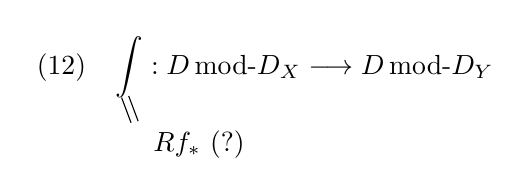
\begin{tikzpicture}
\node[anchor=west] at (-1,0) {$(12)$};
\node[anchor=west] at (0,0) {$\displaystyle\int:D\,\mathrm{mod}\text{-}D_X\longrightarrow D\,\mathrm{mod}\text{-}D_Y$};
\draw (0.20,-0.38)--(0.32,-0.70);
\draw (0.29,-0.36)--(0.41,-0.68);
\node[anchor=west] at (0.48,-0.98) {$R f_*\ (?)$};
\end{tikzpicture}
\end{adjustbox}
\end{center}

\begin{equation*}
\int\mathcal{M}=R f_{\bullet}\left(\mathcal{M}\underset{D_X}{\overset{L}{\otimes}}D_{X\to Y}\right)
\qquad\text{— комплекс}
\tag{13}
\end{equation*}
\Unclear{GELFAND-P000939}{equation-thirteen-cancelled-subscript}{[В индексе у $D$ под $\otimes$ зачёркнут знак: $Y$? / $X$?; ниже вписано $X$.]}

\begin{equation*}
\int^i\mathcal{M}=H^i\left(\int\mathcal{M}\right)
\tag{14}
\end{equation*}

(Sato, Kashiwara)

(15) \underline{Теорема}. $Y$ — точка $\Rightarrow$

\Unclear{GELFAND-P000939}{last-formula-number}{[Номер следующей формулы: (16) / (15).]}
\begin{equation*}
\int^i\omega_X=H^{\dim X+i}(X)
\end{equation*}
\Unclear{GELFAND-P000939}{last-exponent-cancellation}{[Перед $\dim X+i$ в показателе у $H$ зачёркнут знак: $2$?]}

($X$ — неособое над $\mathbb{C}$)

\SourcePage{GELFAND-P000940}{25}
\underline{С. Гельфанд}

\underline{Производные категории.}

\underline{Зад. 1.} Если есть 2 компл. с изом. когомологиями, то не всегда можно
изом. когом. прод. до отобр. компл., индуц. изоморфизм.

\underline{Зад. 2.} Рассм. сферу $S^n$ и на ней кат. пучков аб. групп $C$. На ней
действ. $O(n)$. Рассм. кат. с действ. \Unclear{GELFAND-P000940}{top-action-abbreviation}{гр.}
и произв. кат. $D(C)$. Рассм.
двойств. $S^{*n}$. $C_1$
\Unclear{GELFAND-P000940}{top-cancelled-symbol}{зачёркнутый знак: неразборчиво}

$C_1$ не изом. $C$ (действие другое)
\begin{equation*}
\underline{\underline{D(S)\sim D(S^*)}}\quad!!
\end{equation*}

\underline{24.11.80г}\qquad\underline{сем. Гельфанда.}

% Left-hand timetable region.
\underline{Секционные.}

\underline{25}

\Unclear{GELFAND-P000940}{section-room-prefix}{к.} $\underrightarrow{451}$
\Incomplete{GELFAND-P000940}{section-cancelled-entry}{Неразборчивая зачёркнутая запись перед временем первого выступления.}

$15^{00}$ Сергеев

$15^{20}$ \underline{Mebkhout} (France)

\quad зад. Рим.-Гильб. в высш. размер.

$15^{40}$ Хенкин

$16^{00}$ \underline{Kantor} J.-M.

% Boxed right-hand conference timetable; its date groups are distinct from the left column.
\fbox{\parbox{12cm}{
\underline{Конфер.}\newline
\underline{\underline{Пленарные.}}\newline
\underline{24.}\quad $16^{20}$ Sato\newline
\underline{25.}\quad $10^{00}$ Morimoto\newline
\hspace{1cm}$10^{40}$ Маслов\newline
\hspace{1cm}$11^{40}$ Gesztelyi\newline
\hspace{1cm}(обобщ. ф-и в ур. \Incomplete{GELFAND-P000940}{gesztelyi-note-ending}{Неразборчивое окончание после «в ур.»; видимое начало допускает «ча», возможное чтение «частн.»; закрывающая скобка не видна.}\newline
\hspace{1cm}$12^{20}$ Березанский и др.\newline
\underline{26.}\quad \Incomplete{GELFAND-P000940}{conference-cancelled-time}{Зачёркнутая запись времени перед 10.00 не читается.} \underline{10.00}\quad\underline{Laugwitz}\newline
\hspace{1cm}(с нестанд. т. зрения)\newline
\hspace{1cm}$10^{40}$ \underline{Иванов}\newline
\hspace{1cm}$11^{40}$ \underline{Хромов}, \underline{Данилов}\newline
\hspace{1cm}$12^{20}$ \underline{Berg}\quad умнож. распр.\newline
\underline{28.}\quad $10^{00}$ \underline{Lions}\newline
\hspace{1cm}$10^{40}$ \underline{Гельфанд}\newline
\hspace{1cm}$11^{40}$ \underline{Komatsu} — ядра в ультрараспред.\newline
\hspace{1cm}$12^{20}$ \underline{Lassner}\newline
\hspace{1cm}$13^{00}$ \underline{Жаринов}
}}

% Lower left region, below the sectional timetable.
\underline{Д.Б. Фукс.}\qquad\underline{Умн. Уайтхеда}
\begin{equation*}
\pi_n(X)\times\pi_m(X)\longrightarrow\pi_{n+m}(X)
\end{equation*}
$\sim$ коммутатор в алг. Ли
\begin{equation*}
\partial(I_n\times I_m)=(\partial I_n\times I_m)\cup(I_n\times\partial I_m)
\end{equation*}
Тождество Якоби есть — \Unclear{GELFAND-P000940}{fuchs-final-abbreviation}{суперсим.} Ли!!

\underline{\underline{В. Ломоносов.}}

$(A-A')$ — ядерный

$B$ комм. с $A$, $B'$ комм. с $A'$; $(B-B')$ — вп. непр
\begin{equation*}
\Rightarrow\quad B|_{\mathcal H_{ac}(B)}\underset{\text{унит.}}{\sim}B'|_{\mathcal H_{ac}(B')}
\end{equation*}
$\Rightarrow$ теор. расс. сразу для коммут. сем-в операторов.

\underline{\underline{А. Бейлинсон.}}

\begin{adjustbox}{max width=\linewidth}
\begin{tikzcd}
X \arrow[r,"f"] & Y
\end{tikzcd}
\end{adjustbox}

\begin{equation*}
(1)\qquad f^*:\mathcal D_Y\text{-}\mathrm{mod}\longrightarrow\mathcal D_X\text{-}\mathrm{mod}
\end{equation*}
Введём
\begin{equation*}
f_*:\mathrm{mod}\text{-}\mathcal D_X\longrightarrow\mathrm{mod}\text{-}\mathcal D_Y
\end{equation*}
% Bracketed note to the right of (1); “на Y” is an interlinear insertion.
\begin{equation*}
\left[\begin{aligned}
&\text{если }\overset{\text{на }Y}{u}\text{ уд. сист. }M,\\
&\text{то }f^*u\text{ уд. сист. }f^*M
\end{aligned}\right.
\end{equation*}
\begin{equation*}
(2)\qquad\mathcal D_{X\to Y}=f^*(\mathcal D_Y)\in\mathcal D_X\text{-}\mathrm{mod}\text{-}\mathcal D_Y
\qquad\text{(бимодули)}
\end{equation*}
\begin{equation*}
(3)\qquad f_*M=f_\bullet(M\otimes_{\mathcal D_X}\mathcal D_{X\to Y})
\end{equation*}
($\underset{\text{если}}{f_*}$ на формах объёма с комп. носителем)

% Bracketed lower-right note and its small insertion above “u на X”.
\Unclear{GELFAND-P000940}{lower-right-omega-insertion}{вставка над «$u$ на $X$»: $\in\Omega_1(X)$ или $\in\Omega_c(X)$}
\begin{equation*}
\left[\begin{aligned}
&\text{если }u\text{ на }X\text{ уд. сист. }M,\\
&\text{то }f_*u\text{ уд. сист. }f_*M
\end{aligned}\right.
\end{equation*}

\SourcePage{GELFAND-P000941}{unlabelled}
(Сист. ур-й, к-рой удовл. несобственные интегралы)

\begin{equation*}
(4)\qquad f_*\text{ не функториально:}\qquad(fg)_*\ne f_*g_*
\end{equation*}
Строим.
\begin{equation*}
(5)\qquad Rf_*:D(\mathrm{mod}\text{-}D_X)\longrightarrow D(\mathrm{mod}\text{-}D_Y)
\end{equation*}

\underline{Пример:} $X$ — плоскость, $Y$ — прямая, $f$ — проекция,

$M$ — пучок форм на $X$ (старшей степени)
\begin{equation*}
Rf_*(M)\text{ — комплекс,}\qquad
\begin{aligned}
&0\text{-комп. — }0\\
&(-1)\text{-комп. — }\underline{\text{формы на прямой.}}
\end{aligned}
\end{equation*}
\begin{equation*}
(6)\qquad Rf_*(M)=Rf_\bullet(M\overset{L}{\otimes}_{\mathcal D_X}\mathcal D_{X\to Y})
\end{equation*}
$\overset{L}{\otimes}$ — левый произв. функтор от тенз. произвед.

$Rf_\bullet$ — правый произв. функтор от функтора (!) $f_\bullet$

(7)\qquad\underline{Предл.}

\begin{adjustbox}{max width=\linewidth}
\begin{tikzcd}
X\arrow[r,"f"]&Y\arrow[r,"g"]&Z
\end{tikzcd}
\end{adjustbox}
\begin{equation*}
\begin{gathered}
\Downarrow\\
Rg_*Rf_*=R(g\circ f)_*
\end{gathered}
\end{equation*}
\Unclear{GELFAND-P000941}{cancelled-word-before-parenthesis}{зачёркнуто: (так}
($f_*$ не облад. этим св-вом)

Пусть
\begin{equation*}
M\in\mathrm{mod}\text{-}\mathcal D_X
\end{equation*}
\begin{equation*}
(8)\qquad\ldots\longrightarrow M\otimes\Lambda^2T_X\longrightarrow M\otimes T_X\underset{\nearrow}{\longrightarrow}M
\end{equation*}
% The short upward-right pointer in the source connects the following right-hand note to the last differential.
($T_X$ — касат. пучок к $X$)\qquad(т.к. $M$ — правый $\mathcal D_X$-mod, $T_X\subset\mathcal D_X$)

(9)\qquad\underline{Предл.}

\underline{Рассм. когомологии} (8). \underline{Они совпад. с когом. компл. (6)}, т.е.

\quad(де Рама!)
\begin{equation*}
(10)\qquad R\Gamma(\underbrace{DR}_{\text{De Rham}}M)=Rf_*(M)
\end{equation*}
(\underline{здесь} $f:X\longrightarrow\underline{\text{точка}}$).

$M$ — пучок форм объёма $\Rightarrow$ (8) — обычный компл. де Рама, но
сдвинутый на \Unclear{GELFAND-P000941}{de-rham-shift-amount}{$M$ или $n$} влево

% The source has a short unheaded sloping pointer from the volume-form note toward omega.
\begin{adjustbox}{max width=\linewidth}
\begin{tikzpicture}[baseline=(formula.base)]
\node (formula) at (0,0) {$(11)\qquad R^if_*\omega=H^{\dim X+i}(X)$};
\node[anchor=west] at (-0.8,0.8) {\small пучок всех форм объёма};
\draw (-1.35,0.22) -- (-0.95,0.52);
\end{tikzpicture}
\end{adjustbox}

Более общ.: \underline{Для гладкого морфизма — пучки когом. вдоль слоёв!}
\begin{equation*}
(12)\qquad\ldots\longrightarrow M\otimes\Lambda^2T_{X/Y}\longrightarrow M\otimes T_{X/Y}\longrightarrow M
\quad\longleftarrow\quad(\text{это }DR_{X/Y}M)
\end{equation*}

\SourcePage{GELFAND-P000942}{26}
Тогда
\begin{equation*}
(13)\qquad Rf_\bullet(DR_{X/Y}M)=Rf_*(M)
\end{equation*}
% “относит.” is inserted above the beginning of the DR-complex phrase.
Итак, в прямом образе \textit{[Над началом следующей записи вписано: относит.]}
\Unclear{GELFAND-P000942}{relative-dr-complex-word}{$DR$компл.}
ввод. \underline{действие дифф. операторов} (!)

(не очевидно, т.к. в исх. пучке
\Unclear{GELFAND-P000942}{overwritten-word-before-net}{его; надпись сверху: д.?}
нет). Это действие назыв.

\underline{связностью Гаусса-Манина.}

\underline{2-й случай}

\begin{adjustbox}{max width=\linewidth}
\begin{tikzcd}
X\arrow[r,"f"]&Y
\end{tikzcd}
\end{adjustbox}
\underline{вложение.}
\begin{equation*}
\begin{aligned}
(14)\qquad Rf_*(M)&=Rf_\bullet(M\overset{L}{\otimes}_{\mathcal D_X}\mathcal D_{X\to Y})\\
&=f_\bullet(M\overset{L}{\otimes}_{\mathcal D_X}\mathcal D_{X\to Y})=
\end{aligned}
\end{equation*}
(Функтор $f_\bullet$ в этом случае точен —)

\quad — не возник. когом. вдоль слоёв
\begin{equation*}
=f_\bullet(M\otimes_{\mathcal D_X}\mathcal D_{X\to Y})
\end{equation*}
(т.к. $\otimes$ в этом случае точен)

$\omega\rightsquigarrow$ формы, прод. $\delta$-ф-ями в трансверс. направл.

\underline{Голономные модули.}

$X$ — мн-ие, $M$ — конечно порожд. $\overset{\mathcal D_X\text{-}}{\text{модуль}}$
\Unclear{GELFAND-P000942}{cancelled-module-end}{зачёркнуто: $M$?}

Он наз. \underline{голономным}, если $\forall x\in X$,
\begin{equation*}
\underline{\text{когомологии}}\quad Li_x^*M\quad\underline{\text{конечномерны}}
\end{equation*}
\quad(слой модуля над точкой)

\SourceFigure{GELFAND-P000942}{point-inclusion-diagram}{Справа от определения в скобках изображена направленная вправо стрелка включения с надписью $i_x$ сверху; справа $X$, слева $x$ с неясным дополнительным знаком перед ним. Под рисунком написано «вложение».}

($i_x^*M$ — «замораживание коэфф.» — см. выше)

$\sim$ комплекс $Li_x^*M$ конечномерен (т.к. в произв. категории).

\underline{Своб. модуль}\quad\underline{не явл. голономным} (см. прошл. раз)

Голономность $\sim$ переопределённость.

\underline{Примеры}

% The expression X=... is inserted above the beginning of example а).
а) \Unclear{GELFAND-P000942}{example-a-field}{$X=C^1$ или $X=R^1$}
рассл. с интегр. связностью

Модуль так устроен, кроме конечн. числа точек, где могут быть
особ.

б) $X=C^2$ опять на доп. к конечн. числу
\Unclear{GELFAND-P000942}{example-b-cancelled-word}{зачёркнуто: точек}
% “кривых” is the replacement inserted above the cancelled word.
кривых — рассл. с интегр.
связн. На этих кривых — особенности.

\tikz[baseline=(question.base)]{\node[draw,circle,inner sep=2pt] (question) {?};}
\underline{Все получ. склейкой} из модулей, получ. из $\delta$-ф-й по нормали.

\textit{[Зачёркнуто:}
(кроме \Unclear{GELFAND-P000942}{last-cancelled-middle}{точек самих; точек этих}
кривых \Incomplete{GELFAND-P000942}{last-cancelled-tail}{Неразборчивое окончание зачёркнутой строки после «кривых».}
\textit{]}

\SourcePage{GELFAND-P000943}{unlabelled}
(15) \underline{Теор.} 1) $\forall$ \underline{голон. модуль имеет конечную длину}
(фильтрации с непр. факторами им. од. длину)

2) \underline{есть опис. всех неприводимых}

\begin{equation*}
Y\subset X,\qquad Y\text{ непривод.}
\end{equation*}

Непривод.\ 
\begin{adjustbox}{max width=\linewidth}
\begin{tikzpicture}[baseline=0pt]
\node[inner sep=2pt] (insert) at (0,0.5) {\small плоское};
\draw (0,0.5) ellipse (0.63 and 0.26);
\draw (insert.south west) .. controls (-0.15,0.2) and (-0.03,0.1) .. (0,0);
\draw (0,0) .. controls (0.07,0.25) and (0.2,0.3) .. (insert.south east);
\end{tikzpicture}
\end{adjustbox}
рассл. $\mathcal L_Y$ со связностью на $Y$
(векторное рассл. с интегр. св.)

2 пары $Y_1,Y_2$ наз. эквив., если $Y_1$ открыто в $Y_2$
и
\begin{equation*}
\mathcal L_{Y_1}=(\mathcal L_{Y_2})\big|_{Y_1}
\end{equation*}
(можно выброс. замкн. подмн-ва, зад. над общей точкой)

(16) \underline{\underline{Утв.}} $i:Y\hookrightarrow X$

\underline{В $i_*\mathcal L_Y$ \underline{есть единств. неприв. подмодуль.}}

это и есть искомый объект --- непривод. модуль

$Y$ --- гладкое $\Rightarrow$ уже неприводимо

В особ. появл. $\delta$-ф-и.

\begin{adjustbox}{max width=\linewidth}

\begin{tikzpicture}[x=1cm,y=1cm]
\fill (-1.3,-0.08) -- (-0.28,0.12) -- (-0.28,-0.04) -- cycle;
\fill (0,0.02) circle (0.09);
\fill (0.3,0.13) -- (1.34,0.07) -- (0.3,-0.04) -- cycle;
\end{tikzpicture}
\end{adjustbox}

\SourcePage{GELFAND-P000944}{27}
\begin{adjustbox}{max width=\linewidth}
\begin{tikzpicture}[baseline=(date.base)]
\node[anchor=west,inner sep=0pt] (date) at (0,0) {$1/\underline{\overline{\mathrm{XII}}}$-80 г.};
\draw (0,-0.22) rectangle (2.45,-0.36);
\draw (0.32,-0.22) -- (0.28,-0.36);
\draw (0.66,-0.22) -- (0.62,-0.36);
\draw (1.02,-0.22) -- (0.98,-0.36);
\draw (1.38,-0.22) -- (1.34,-0.36);
\draw (1.75,-0.22) -- (1.71,-0.36);
\draw (2.10,-0.22) -- (2.06,-0.36);
\end{tikzpicture}
\end{adjustbox}
\quad \underline{Сем. Гельфанда.}

\underline{С. П. Новиков.}

(1)
\begin{equation*}
\hat H=\text{\Incomplete{GELFAND-P000944}{equation-one-cancellation}{Неразборчивая зачеркнутая запись перед дробью.}}
\frac12\sum_{\alpha=1}^n\left(i\frac{\partial}{\partial x^\alpha}-eA_\alpha\right)^2+cV(\vec x)
\end{equation*}

(2)
\begin{equation*}
H_{\alpha\beta}=\partial_\beta A_\alpha-\partial_\alpha A_\beta
\end{equation*}
$V$ — эл. поле, $H_{\alpha\beta}$ — магн. поле

(3)
\begin{equation*}
\hat H\psi=\varepsilon\psi\qquad\text{спектр. задача.}
\end{equation*}

Интересен случай, когда

(4) $H_{\alpha\beta}(x)$ и $V(x)$ период. с решеткой периодов.

\begin{adjustbox}{max width=\linewidth}
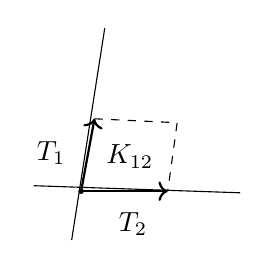
\begin{tikzpicture}[x=1cm,y=1cm]
\draw (-0.6,0.07) -- (2.02,-0.02);
\draw (-0.12,-0.62) -- (0.3,2.07);
\draw[thick,->] (0,0) -- (0.17,0.92);
\draw[thick,->] (0,0) -- (1.1,0);
\draw[dashed] (0.17,0.92) -- (1.22,0.87) -- (1.1,0);
\fill (0,0) circle (0.035);
\node at (-0.38,0.48) {$T_1$};
\node at (0.66,-0.42) {$T_2$};
\node at (0.62,0.44) {$K_{12}$};
\end{tikzpicture}
\end{adjustbox}

(не только эл. поле, но и его потенциал;
постоянное эл. поле — \Unclear{GELFAND-P000944}{constant-electric-word}{неразумно / периодично})

— потенциал тогда $\vec E\cdot\vec x$ \Unclear{GELFAND-P000944}{electric-potential-cancellation}{зачеркнутый знак: неразборчиво} —

\underline{— не изучена даже 1-мерн. задача.})

$A_\alpha$ не периодичны (вообще говоря).

$K_{\alpha\beta}$ — ячейка (элем.), нат. \Unclear{GELFAND-P000944}{cell-preposition}{на / по} $\alpha$ и $\beta$ \Unclear{GELFAND-P000944}{cell-coordinate-ending}{координату}

(5)
\begin{equation*}
\iint_{K_{\alpha\beta}}H_{\alpha\beta}\,dx^\alpha\wedge dx^\beta=\Phi_{\alpha\beta}
\qquad\text{— магн. потоки (базисные)}
\end{equation*}
(суммир. нет!)

(6)
\begin{equation*}
i\nabla_\alpha=i\frac{\partial}{\partial x^\alpha}-eA_\alpha
\qquad\text{имеет смысл связности}
\end{equation*}

\underline{Замеч.} Спин здесь 0, со спином $1/2$ будет

(7)
\begin{equation*}
\hat H=(1)+e\sigma_j H^j,\qquad\text{где }H^1=H_{23},\quad H^2=-H_{13},\quad H^3=H_{12};
\end{equation*}
$\sigma_1,\sigma_2,\sigma_3$ — матр. Паули

(8) \underline{Допустимый случай:} $\displaystyle\frac e{2\pi}\Phi_{\alpha\beta}\in\mathbb Z$

Оператор $\hat H$ рассм. в $L^2(\mathbb R^n)$.

(9) $(8)\Rightarrow\hat H$ — универс. накрыв. опер. на торе (в расслоении), \Unclear{GELFAND-P000944}{covering-overwritten-word}{причем}

(10)
\begin{equation*}
\left(c_1(\xi),\underset{\substack{\vert\\\text{баз. цикл}}}{Z_{\alpha\beta}}\right)=\frac e{2\pi}\Phi_{\alpha\beta}
\end{equation*}

Однако опер. всегда имеет смысл (физич.), но теории нет.

(11) Иррацион. \Unclear{GELFAND-P000944}{irrational-final-abbreviation}{инт.} \underline{Рац. свод. к нему укрупнением решетки}

\SourcePage{GELFAND-P000945}{unlabelled}
\begin{adjustbox}{max width=\linewidth}
\begin{tikzpicture}[baseline=(heading.base)]
\node[anchor=west,inner sep=0pt] (heading) at (0,0) {Магнитные трансляции.};
\draw[dashed] (0,-0.16) -- (4.65,-0.16);
\end{tikzpicture}
\end{adjustbox}

\underline{2 типа задач.} а) \Unclear{GELFAND-P000945}{top-cancelled-abbreviation}{зачеркнуто: магн.} реш. навязана (тв. тел!), а магн. поле извне

б) типа сверхпров.: магн. поле само возникает,
они автоматич. целочисл.

а) $K_{\alpha\beta}\sim10^{-10}\text{ см}^2$ \qquad б) $\sim10^{-16}\text{ см}^2$

\underline{Магн. трансл.} Имеем:

(12)
\begin{equation*}
A_\alpha(\ldots,x^i+T_i,\ldots)=A_\alpha(x)+\partial_\alpha f_i
\end{equation*}
(т.к. $dA$ периодичен)

(13)
\begin{equation*}
\hat T_j^*\psi(x)=\psi(..\,x^{\Unclear{GELFAND-P000945}{translation-coordinate-superscript}{i / t}}+T_j,\,)\exp(-ie f_j)
\end{equation*}
(опер. магн. трансляции)

(14) \underline{Лемма 1} (известная $\sim$60-е годы\Unclear{GELFAND-P000945}{lemma-cancelled-character}{зачеркнутый знак: неразборчиво}, \underline{Зак и Браун})

\begin{equation*}
\hat T_j^*\hat T_k^*=\hat T_k^*T_j^*\exp(-ie\Phi_{kj}),\qquad j,k=1,\ldots,n.
\end{equation*}

Получилось проективное предст. аб. группы, коциклы заранее заданы.

Иррац. потоки $\Rightarrow$ получ. группы не типа 1. (подгр. в гр. Гейзенберга).

(15)
\begin{equation*}
\frac{e\Phi_{kj}}{2\pi}\in\mathbb Z\Rightarrow\text{коммут. группа}
\end{equation*}

$\underline{n=2}$

($n=3$ тоже интересно)

сверхпров. — 2-мерн. задача

\underline{Задача:} описать спектр $\hat H$.

(16) $[\hat H,\hat T_j^*]=0\Rightarrow$ соб. ф-и надо искать одновр. собств. для $\hat T_j^*$

\Unclear{GELFAND-P000945}{eigenfunction-cancelled-abbreviation}{зачеркнуто под строкой: магн.}

Магнито-блоховские:

(17)
\begin{equation*}
\hat T_j^*\psi_{\Unclear{GELFAND-P000945}{bloch-subscript-left}{p}}=\exp(ip_jT_j)\psi_{\Unclear{GELFAND-P000945}{bloch-subscript-right}{p}}
\end{equation*}

Опер. в $L^2$ = прямой инт. опер. на торе с такими гран. усл.

$p_j$ — \underline{квазиимпульсы} \qquad $(p_1,p_2)\in\mathbb T^2$ \qquad (тор обр. решетки)

Фиксируем $p_1,p_2\Rightarrow$ опер. в рассл. на торе с об. усл.

(18)
\begin{equation*}
\varepsilon_j(p_1,p_2)\qquad\text{— закон дисперсии}
\end{equation*}
\begin{equation*}
j=1,2,\ldots
\end{equation*}

\SourcePage{GELFAND-P000946}{28}

(19) \underline{Теорема}. \underline{Пусть} $V=0$, \underline{спин} $s=\frac12$,
\begin{equation*}
n=2,\qquad N\underset{\mathrm{def}}{=}\frac{e\Phi_{12}}{2\pi}.
\end{equation*}

\begin{flushright}
[На правом поле, отделено двойной вертикальной чертой:]\\
Дубровин, Новиков\\
ЖЭТФ, сент. 1980.\\
и ещё есть раб. в ДАН
\end{flushright}

(магн. поле напр. по оси $Z$ — 2-мерн. случай — и период.)

\underline{Тогда} \underline{задав} $A=(a_1,\ldots,a_N)\in C^N$, \underline{мы} \underline{получим}, \underline{что} \underline{соб.} ф-я \underline{им. вид}
[над «соб.» вписано, с фигурной связкой к строке: $(\forall\ \text{магн.-блох.})$]
\begin{equation*}
\Psi_A=\exp(-e\varphi)\prod_{j=1}^N\sigma(z-a_j)\exp(-az);\tag{20}
\end{equation*}

\begin{flushright}
($\sigma$ — элл. ф-я Вейерштрасса)\\
одна из $\theta$-ф-й
\end{flushright}

\begin{equation*}
p=p_1+ip_2=\frac{2\pi i}{T_1T_2}\sum a_j+\operatorname{const}(H),\tag{21}
\end{equation*}
[Под $\operatorname{const}(H)$, с указательной чертой:] зав. от магн. поля.
\begin{equation*}
\mathcal D=\sum a_j.\qquad\text{(дивизор)}
\end{equation*}

(22) [Зачёркнуто: \Unclear{GELFAND-P000946}{eq22-cancel}{запись перед $\varphi(x,y)$; возможно, $\varphi(x,y)$}.]
\begin{equation*}
\varphi(x,y)=\frac{1}{2\pi}\int_{K_{12}}\ln|\sigma(z-z')|H(z')\,d^2z'.
\end{equation*}
$z={}$[зачёркнуто: \Incomplete{GELFAND-P000946}{z-cancel}{Многознаковая зачёркнутая запись после знака равенства не читается.}]${}\,x+iy$.

Ф-и (20) — полный базис решений ур-я $\hat H\psi=0$

(точная \Unclear{GELFAND-P000946}{exact-abbr}{информ. / интегр.} на нижнем нулевом ур. энергии)

[Зачёркнуто: $L^2=(L^2)^0+{}$\Incomplete{GELFAND-P000946}{l2-cancel}{Окончание зачёркнутой формулы после плюса не читается.}]
\begin{equation*}
L_2=L_2+L_2^\perp.
\end{equation*}
\Unclear{GELFAND-P000946}{l2-split}{над первым $L_2$ справа видна петля у нижнего выносного штриха «ур.» предыдущей строки; возможны $L_2$ и $L_2^0$}.

\begin{equation*}
a=a(a_1,\ldots,a_N)\quad\text{— \underline{вычисляется}}.\tag{23}
\end{equation*}

Выделение завис. (23) — это выдел. вещ. \underline{квазиимпульсов}

(ф-я $\Psi_A$ всегда собств. и блоховская).

$\lambda\Psi_A$ тоже соб. ф-я

$(\lambda,a_1,\ldots,a_N)$ — полное мн-во параметров.

\underline{Замеч.}
\begin{equation*}
(\lambda,a_1,\ldots,a_N)\overset{P}{\longrightarrow}\mathbb T^2.\tag{24}
\end{equation*}

(25) Получ. [зачёркнуто: \Incomplete{GELFAND-P000946}{eq25-cancel}{Плотно зачёркнутая запись не читается; исходное число знаков установить нельзя.}] \underline{голом. вект. рассл.} ($N$-мерное) на $\mathbb T^2$ с $\underline{c_1=N}$.

(= число квантов магн. потока)

(26) \underline{Слой} — при фикс. $p$ — получ. $\underline{\underline{\mathcal L(\mathcal D)}}$, $\dim\mathcal L(\mathcal D)=N$

[Зачёркнуто: \Unclear{GELFAND-P000946}{eq26-cancel}{возможно, «Далее»}.]
(умнож. на двоякопер. ф-ю)

\begin{flushright}
$\mathcal D$ — дивизор нулей $\sigma$\\
$\mathcal D=\sum a_j$\\
(дивизор)
\end{flushright}

На самом деле (26) — из теор. Атия-Зингера
\begin{equation*}
(\operatorname{Coker}=0)
\end{equation*}
бесконечномерный аппарат.

\underline{Магн. поле при этом:}
\begin{equation*}
A_1=-\partial_2\varphi,\quad A_2=\partial_1\varphi,\quad\Delta\varphi=H.\tag{27}
\end{equation*}

$a_1,\ldots,a_N$ опред. mod решётки и симметризованы, т.е.
\begin{equation*}
a\in S^N\Gamma.
\end{equation*}

\SourcePage{GELFAND-P000947}{unlabelled}

Слой (25) — лин. пр-во. (не очевидно сразу)

Все ф-и $\Psi_A$ в фиксир. слое получ. из одной умн. на \Unclear{GELFAND-P000947}{top-elliptic}{эллипт. / эллип.} 2-пер. ф-и.

\underline{Следствие:} блох. ф-и обр. образ. линейное расслоение.

\underline{Соб. ф-и при фиксир. $p$ образуют $N$-мерное пр-во (!)}

(\underline{размерн. фиксирована})

В однор. магн. поле \underline{утв. верно} для всех ур. энергии.

[Зачёркнуто: \underline{Вопрос 2.} Откуда вырождение?]

Теперь возмутим:
\begin{equation*}
\hat H=\hat H_0+e\,v(x,y)\qquad\text{(с той же гр. периодов).}\tag{28}
\end{equation*}

(29) \underline{Теорема 2}. \underline{Возмущ. опр.} — \underline{квадр. форма общего} \underline{типа}.

(2-пар. сем-во квадр. форм общего пол. среди всех компл. эрмитовых форм).

Т.е. если исключить мн-во потенц., на коэфф. Фурье к-рых наложены 3 ур-я, то спектр (блох. соб. ф-и) облад. след. св-вами
\begin{equation*}
\hat V_{(p_1,p_2)}(\Psi_A)=\iint_{K_{12}}\bar\Psi_A\,v\Psi_A\,dx\,dy.\tag{30}
\end{equation*}

(компл. эрмитова форма, $\Psi_A$ — соб. ф-и $H_0$)

при фиксир. квазиимпульсах.

(30) Нах. в общем положении (как оператор)

Квадр. форма общего полож. — ни одна пара соб. [зачёркнуто: \Unclear{GELFAND-P000947}{eigen-cancel}{возможно, «ф-и»}] чисел не сливается

Отобр. тора в мн-ве квадр. форм — \underline{в общем положении}.

(В 1-мерн. случае — никогда не бывает в общем положении)

из-за того, что опер. 2-го порядка.

([Зачёркнут знак: \Unclear{GELFAND-P000947}{codim-firstmark}{возможно, $\Rightarrow$}; ниже вписано: т.к.] коразм. 3,
[зачёркнуто: \Unclear{GELFAND-P000947}{codim-cancel-top}{возможно, «то»}] то не пересек. с кратн. соб. знач.,

$\underline{\underline{n=3}}$ [зачёркнуто: \Unclear{GELFAND-P000947}{codim-cancel-left}{возможно, «коразм. 2»}] $\Rightarrow$
[зачёркнуто: \Incomplete{GELFAND-P000947}{codim-cancel-right}{В записи после стрелки различимо начальное «в»; остальные буквы закрыты штрихами.}]
пересек. в изолир. точках.)

\underline{\underline{Следствие:}}

$\underline{n=2}\quad\Rightarrow$ расслоение расп. на 1-мерные

\underline{\underline{И.М.Г.:}}

Интересен иррац. случай!

(там всё на самом деле некоммутативно)

Идея: войти в компл. область (внутри круга!) — в несамосопр. ситуации

т.е. сделать \underline{регуляризацию} (параболич.)

\SourcePage{GELFAND-P000948}{29}

\underline{Иррац. случай:}
\begin{equation*}
H_{12}=\frac{\partial A_1}{\partial x_2}-\frac{\partial A_2}{\partial x_1},\qquad A_1\,dx_1+A_2\,dx_2.
\end{equation*}
\begin{equation*}
\left[\left(i\frac{\partial}{\partial x_1}-A_1\right)^2+\left(i\frac{\partial}{\partial x_2}-A_2\right)^2\right]=\hat H.
\end{equation*}
\begin{equation*}
H_{12}(x_1+m_1T_1,x_2+m_2T_2)=H_{12}(x_1,x_2)
\end{equation*}
\begin{equation*}
\Phi_{12}=\iint H_{12}\,dx_1\wedge dx_2.
\end{equation*}
\begin{equation*}
\Phi_{12}\ne2\pi\frac{N}{M}
\end{equation*}

\underline{Группа:}
\begin{equation*}
\hat T_1^*\hat T_2^*=\hat T_2^*\hat T_1^*\exp(-i\Phi_{12})
\end{equation*}
действует в мн-ве всех ф-й (фиксир. соб. [зачёркнуто: \Incomplete{GELFAND-P000948}{subspace-cancel}{Буквенная запись между «соб.» и «подпр-ве» закрыта плотной штриховкой.}] подпр-ве)

$[H,\hat T_j^*]=0$ по-прежнему (подбор $f_j$ в (12)-(13)).

В основе теории [над строкой вписано, со связкой после «теории»: факторов] фон Неймана — \underline{неприводимость эргодичность}.

\underline{И.М.Г.} К следующему семестру знать: $G$-структуры, $D$-структуры и резольвенту Спенсера.


\SourcePage{GELFAND-P000949}{51}
% Original scan: 2440 x 3480 pixels. Coordinates below use a top-left origin.
% Review boxes (x0,y0,x1,y1), nearest-neighbour enlargement:
% header (170,30,1190,360) 3x; problem (280,350,1790,590) 3x;
% embeddings (330,585,1460,1120) 3x; want (320,1120,1710,1410) 3x;
% geodesics (310,1390,1960,1860) 3x; hypersimplex (300,1840,1300,2335) 3x;
% definition (340,2330,2270,2860) 3x; bottom (170,2900,2390,3410) 3x.
% Resolved details: полиэдры (975,345,1280,445) 8x, independently reread;
% Наивный способ (435,1330,880,1425) 5x; координ. (1100,3105,2355,3200) 3x.
% Independent check: lower G_1^3 (925,925,1045,1035) 10x;
% Rank sign (405,1760,725,1855) 8x; doubled-stem upper R (1020,600,1310,735) 6x;
% comma and lower R (395,2005,1050,2190) 5x;
% Грассм. in heading (575,2350,1160,2455) 5x; later Грасм. (410,2925,875,3030) 5x;
% underline endpoints (190,35,700,265) 5x.

\underline{\underline{9/II-81}}.\qquad \underline{Сем. Гельфанда.}

\underline{MacPherson}.

(\underline{О совм. раб. с И. М. Гельфандом.})

Зад. — найти интересные полиэдры в грассманианах.

В проект. пр-вах многогранники имеют \underline{плоские} грани
(грань $\subset$ подпр-ве меньшей разм.)

\begin{gather*}
(0)\qquad P_1\subset P_2\subset P_3\subset\ldots
\end{gather*}
(проективные)

$G_n^m$ — $n$-плоск. в $\mathbb{R}^{m+n}$
(подпр-ва)

Вложения:
\begin{gather*}
(1)\qquad
\begin{array}{ccccccc}
G_1^1&\subset&G_1^2&\subset&G_1^3&\subset&\ldots\\
\cap&&\cap&&\cap&&\\
G_2^1&\subset&G_2^2&\subset&\Unclear{GELFAND-P000949}{embeddings-lower-index}{G_1^3}&\subset&\ldots
\end{array}
\end{gather*}
и т. д.

Хотим: грани — многогр. в меньших

Картина (0) соотв. верхн. строке (1).

Наивный способ:

\SourceFigure{GELFAND-P000949}{geodesic-triangle}{Треугольник с волнистыми сторонами; из левой вершины к правой стороне проведён веер линий. Некоторые внутренние штрихи слабые и прерывистые; точное число и соединение этих штрихов требуют проверки по оригиналу. Буквенных подписей нет.}

есть 3-ник из 3-х геодезич.

Как его заполнить?

тоже геод. (отрезками)

Если в грассманиане сделать это, то не выходит.

Здесь получ.
$\mathrm{Rank}\ge 2$

(2) \underline{Опред.}
\underline{Гиперсимплекс $\Delta_n^m$}: мн-во точек
\begin{gather*}
(x_1,\ldots,x_{n+m})\in\mathbb{R}^{n+m},
\end{gather*}
удовл. соотн.
\begin{gather*}
0\le x_i\le 1,\\
\sum_i x_i=n
\end{gather*}
[После $n$ зачёркнуто: \Unclear{GELFAND-P000949}{hypersimplex-cancellation}{$+1$ / $+m$}.]

(3) \underline{Опр.}\qquad \underline{Грассм. комплекс} в $P_{n+m-1}$:

выбир. $n+m$ точек $e_1,\ldots,e_{n+m}$, не леж. в гиперподпр-ве
меньшей размер. (гиперплоскости).

$H^0$ = связная комп. 1 подгруппы $PGL(n+m)$,
к-рая ост. эти точки на месте.

Грасм. комплекс — замыкание орбиты \underline{общ. полож.} группы $H^0$,
действующей на $G_n^m$.

[Под «общ. полож.» написано: generic.]

(4) \underline{generic — ?}

это значит $H^0\xi$

$\xi$ — подпр-во, трансверс. всем координ. подпр-вам:

если $e_1,\ldots,e_{n+m}$ принять за базис (какие-то точки на них)

это не то же самое, что $\dim=\max$ (!)

\SourcePage{GELFAND-P000950}{unlabelled}
% Original inspected at 2440 x 3480. One visible leaf; no page label seen.
% Coordinates below are (x0,y0,x1,y1) in original pixels, top-left origin.
% Whole-text review boxes: top (170,35,1810,440) 3x;
% diagrams-top (170,450,1085,1270) 3x; collineation (1170,940,1990,1110) 4x;
% example-text (330,1250,2320,1565) 3x; simplex-text (390,1600,1720,1995) 3x;
% dual-picture (355,1990,1020,2785) 3x; dual-text (1100,2030,2380,2470) 3x;
% dual-triangle (1070,2400,2390,2720) 3x; bottom (395,2585,2320,3245) 3x.

(5) \underline{Теорема}.
[Волнистое подчёркивание:] Эти 2 объекта диффеоморфны.

опр. (3) можно пров. для $\forall$ полупрост. группы.

$G_n^m$ — $(n-1)$-подпр-ва в
\Unclear{GELFAND-P000950}{projective-index}{$P_{n+m-1}$ / $P_{m+n-1}$}.

(6) \underline{Пример}.
$\Delta_1^2\qquad G_1^2$

\SourceFigure{GELFAND-P000950}{cube-section}{Куб в перспективе. Слева повторно подписано $\Delta_1^2$. Внутри треугольное заштрихованное сечение с подписью $H$. У верхней левой вершины передней грани стоит $x_2$, у нижней правой — $x_1$; третья подпись, у внутренней нижней левой вершины сечения, похожа на $x_3$ и перекрывается линиями. Видны сплошные и прерывистые рёбра. Третья подпись и точный ход слабых внутренних штрихов требуют сверки с оригиналом.}

\SourceFigure{GELFAND-P000950}{projective-triangle}{Слева $G_1^2$. Треугольник с точками $e_1$ внизу слева, $e_2$ наверху и $e_3$ внизу справа; стороны продолжены за вершины. Центральная область заштрихована и подписана I. Снаружи наверху IV; над левой стороной II, над правой III; за нижней левой вершиной III, за нижней правой II; под нижней стороной IV. У римских чисел видны короткие верхние и нижние горизонтальные черты. Линии местами прерываются около точек; точный ход слабых штрихов и штриховки требует сверки.}

[Волнистое подчёркивание:]
преобр., сохр. \Unclear{GELFAND-P000950}{preserved-symbol}{и / 3} прямые

Внутр. $\Delta$-ка — орбита (и связн. компонента соотв. подгр.)

(т.к. $PGL$ транзит. на 4-ках точек общего положения)

Всего — 4 тр-ка

\SourceFigure{GELFAND-P000950}{hatched-simplex}{Маленький треугольник вершиной вверх. Внутри римское I с верхней и нижней горизонтальными чертами и наклонная штриховка. Тонкие штрихи пересекают подпись либо примыкают к ней; точное число и взаимное положение этих штрихов не установлены.}
— пример грассм. симплекса

Есть гомеом., даже сохр. отрезки (номера)
% Parenthetical номера: (1380,1750,1700,1860), reviewed at 6x.
% Independent check: номера (1395,1750,1715,1865) 8x;
% bottom пересеч. (690,3010,928,3122) 8x;
% inverted triangle (1070,2400,2390,2720) 4x.

$\forall$ ребро — симплекс в $G_1^1$

(7) \underline{Пример}. (другой !!).

$G_2^1$

\SourceFigure{GELFAND-P000950}{dual-orbit-diagram}{Три отмеченные точки: $e_2$ наверху, $e_3$ внизу справа, слева внизу подпись $e_1$ или $e_i$. Через точки проведены пучки прямых; отдельная длинная прямая наклонно пересекает рисунок между верхней и нижними точками. Области над верхней точкой и под двумя нижними заштрихованы. Точные пересечения слабых линий и нижний левый индекс неразборчивы.}

орбита прямой — $\forall$ прямых, не пересек.
заштрих. область.

Это $\Delta$-к — со сторонами —
— прямые, прох. через вершины

% Clear labelled inverted triangle, (1070,2400,2390,2720), reviewed at 3x.
\begin{adjustbox}{max width=\linewidth}
\begin{tikzpicture}[x=1cm,y=1cm]
\draw (0,1.8) -- (1.8,1.8) -- (0.8,0.25) -- cycle;
\node[anchor=south] at (0,1.85) {$13$};
\node[anchor=south] at (1.95,1.85) {$23$};
\draw (0.9,0) ellipse (0.43 and 0.28);
\node at (0.9,0) {$12$};
\node[anchor=west] at (1.7,0) {— соотв. стороне, прох. через $e_1$ и $e_2$};
\end{tikzpicture}
\end{adjustbox}

\SourceFigure{GELFAND-P000950}{small-triangle-curves}{Небольшой треугольник остриём вверх; над верхней вершиной стоит 13. Несколько тонких изогнутых линий пересекают стороны, выходят наружу и образуют петли. Их точное число, взаимное пересечение и ход в слабо пропечатанных участках неразличимы. Других уверенно читаемых подписей нет.}

[Волнистое подчёркивание: Стороны $\in G_1^1$] $\subset G_2^1$

$\Delta_2^1$ — пересеч. куба с плоск. $\sum x_i=2$, причём вершины
тоже обозначены парами.

\SourcePage{GELFAND-P000951}{52}
% Original frame 2440 x 3480; one visible leaf. Heading (210,30,2390,300), reviewed 3x; number (215,45,380,150), 6x.
(8) \underline{Интересный} \underline{пример} $G_2^2$ \underline{или} $\Delta_2^2$

% Cancellation (215,190,380,295), reviewed 7x.
[На левом поле зачёркнуто: \Unclear{GELFAND-P000951}{margin-top-cancellation}{(8) или (9); чтение не установлено}.]
\begin{equation*}
\sum_1^4 x_i=2\quad-\quad
(\perp\ \text{гл. диаг. сечение 4-мерн. куба})
\end{equation*}

% Diagram region (360,275,865,715), reviewed 3x and 5x; margin mark (220,400,320,535), 8x.
[На левом поле зачёркнуто: \Unclear{GELFAND-P000951}{margin-diagram-cancellation}{неразборчивый знак}.]
\SourceFigure{GELFAND-P000951}{diagram-delta}{Рисунок с подписью $\Delta_2^2$. Подписи: $34$ сверху, $24$ справа вверху, $14$ справа ниже, $12$ снизу, $13$ слева, $23$ внутри слева от центра. Видны внешний ломаный контур, сплошные внутренние соединения и короткие прерывистые штрихи. Внутренние соединения у $23$, $24$ и $12$, а также стрелковидные утолщения требуют проверки по оригиналу.}

% Text (335,740,1190,1000), reviewed 3x.
\begin{gather*}
G_2^2\quad-\quad\text{4-мерно}\\
H^0\quad-\quad\text{3-мерно.}
\end{gather*}

% Diagram (480,935,1540,1310), reviewed 3x and 5x.
\SourceFigure{GELFAND-P000951}{diagram-four-planes}{Рисунок с общей нижней левой точкой и линиями к подписям $e_1$ слева вверху, $e_2$ снизу, $e_3$ сверху, $e_4$ справа. Верхняя правая точка подписана $\ell$; к ней идёт средняя наклонная линия из общей левой точки. Видны соединения от областей $e_1,e_2,e_3,e_4$ в сторону $\ell$, часть штрихов прерывистая. Точные соединения слабых линий и характер утолщений у концов требуют проверки по оригиналу.}

% Cross-ratio text (475,1300,2220,1770), reviewed 3x; (495,1310,1165,1490) and (1160,1310,2160,1490), 4x; abbreviation (738,1410,1175,1520), 5x.
$K(\ell)=\text{cross-ratio}$ 4-х плоскостей\newline
\hspace{2em}(ангарм. отнош.)\quad прох. через $\ell$ и выбр. точки

(факторизуем всё по $\ell$ $\Rightarrow$ получ. в плоскости)
\begin{equation*}
H^0\text{-орбита}\ \subset\ K(\ell)=\mathrm{const}
\end{equation*}

% Table (110,1790,1120,2715), reviewed 3x; numbers (400,1805,970,2670), 5x; upper left (195,1785,445,2215), 6x; lower left (115,2410,385,2710), 6x.
\begin{equation*}
\begin{array}{cc}
\begin{gathered}
G_2^2\\
\cup\\
G_2^2\supset
\end{gathered}
&
\left\{\begin{array}{ccc|c}
12&13&14&1\\
21&23&24&2\\
31&32&34&3\\
41&42&43&4
\end{array}\right.
\\
&\rule{11em}{0.3pt}\\
\begin{gathered}
G_2^1\supset\\
\cap\\
G_2^2
\end{gathered}
&
\left\{\begin{array}{ccc|c}
14&42&21&\phantom{1}\\
13&32&21&\\
14&43&31&\\
24&43&32&
\end{array}\right.
\end{array}
\end{equation*}
[\Unclear{GELFAND-P000951}{table-upper-annotation}{В верхней левой вертикальной подписи обе записи читаются $G_2^2$; между ними U-образный знак.}]

% Text (410,2700,1590,2805), reviewed 4x; first word (420,2710,655,2790), 8x; abbreviation (1005,2710,1175,2800), 8x.
Каждое --- в своём \Unclear{GELFAND-P000951}{below-table-abbreviation}{мн-зии / мн-гии / мн-ии} $K(\ell)=\mathrm{const}$

% Theorem heading and line (155,2815,2435,2955), reviewed 3x and 4x; abbreviation (850,2820,1370,2960), 5x; грассм. (1810,2830,2095,2955), 6x.
(9) \underline{Теорема}. Объём мн-ва, закл., между 2-мя грассм. симплексами
\begin{equation*}
K(\ell)=c_1,\quad K(\ell)=c_2
\end{equation*}
равен
\begin{equation*}
\Phi(c_1)-\Phi(c_2),
\end{equation*}
% Difference (520,3070,985,3195), reviewed 6x; overwritten second Phi (770,3070,885,3185), 10x; first argument (625,3080,735,3195), 10x.
[\Unclear{GELFAND-P000951}{theorem-phi-difference}{Во втором знаке $\Phi$ наложены штрихи; первоначальное начертание не установлено. Порядок $\Phi(c_1)-\Phi(c_2)$ сохранён.}]
где
% Formula (505,3190,1730,3350), reviewed 4x; L subscript (670,3190,820,3320), 8x, and (1240,3190,1510,3320), 7x. Caption (1700,3280,2295,3400), 4x.
\begin{equation*}
\Phi(x)=L_1(x)-L_1(1-x),\quad
L_1(x)=\sum_{n=1}^{\infty}\frac{x^n}{n^2},\quad
0<c_1<c_2<1
\end{equation*}
\hspace{10em}(интегр. логарифм)

\SourcePage{GELFAND-P000952}{unlabelled}
% Original inspected at full source resolution: 2440 x 3480.
% Reading order: one visible leaf, top to bottom; no separate page label seen.
% 3x review crops, original pixel boxes (x0,y0,x1,y1):
% top10-left (180,0,1170,350); top10-right (1040,0,1650,350);
% item11 (175,355,1700,620);
% item12-left (180,610,1120,1040); item12-right (1030,610,1990,840);
% item13 (155,1100,1850,1320);
% metric-left (275,1310,1170,1740); metric-right (1040,1320,1920,1740);
% atiyah-title (265,1710,1550,1870);
% five-points-left (295,1880,1210,2180); five-points-right (1110,1880,2010,2100);
% ratios (355,2170,1690,2500); item14 (150,2500,1830,2750);
% bottom-left (310,2740,1350,3300); bottom-right (1150,3020,2330,3300).

(10) \underline{Теорема}. Вообще говоря,
[вписано над строкой: комбинаторный] гомеоморфизм
\begin{equation*}
\Delta_n^m \hookrightarrow \text{грассм. комплекс } G_n^m
\end{equation*}
сохр. ещё ряд структур.
% Resolved insertion: (1110,7,1530,82), reviewed at 6x.
% G superscript m: (1340,155,1465,252), reviewed at 10x.

(11) [Зачёркнуто: \underline{Теорема}]
\SourceFigure{GELFAND-P000952}{faces-orbits-diagram}{Слева «Грани», над словом вписано «внутр.». Вправо идёт стрелка с изогнутым началом, над ней «соотв.». Справа «$H^0$-орбиты», между дефисом и словом зачёркнут знак. Ниже слова «орбиты» короткий вертикальный штрих, затем «лежат в $G_i^j$»; наконечник у вертикального штриха неразличим.}
\Unclear{GELFAND-P000952}{faces-orbits-cancellation}{Зачёркнутый знак между «$H^0$-» и «орбиты»: неразборчиво.}
% Cancellation of Теорема: (386,405,695,501), reviewed at 8x.
% Resolved insertion внутр.: (638,350,856,452), reviewed at 8x.
% Resolved лежат в G_i^j: (1290,500,1670,622), reviewed at 7x.

(12)
\begin{align*}
\partial[\Delta_n^m]
&=\sum_{i=1}^{n+m}(-1)^i
\bigl\{[\Delta_n^{m-1}]\mid i\text{-я коорд.}=0\bigr\}-\\
&-\sum_{-1}^{n+m}(-1)^i\bigl\{[\Delta_{n-1}^{m}]
\end{align*}
\Unclear{GELFAND-P000952}{boundary-formula-second-line}{Во второй сумме снизу видно «$-1$»; строка кончается после $[\Delta_{n-1}^{m}]$. Закрывающая фигурная скобка и дальнейшее условие в источнике не видны.}
% The two minus signs at the line break are both present in the source.
% First summand superscript m-1: (1123,632,1299,770), reviewed at 10x.
% Compared directly with m (603,623,685,687) and n (843,603,892,657), both 10x.
% Lower limit of second sum: (488,980,590,1040), reviewed at 10x.

(13) \underline{Теорема}. $\forall$ гарм. форма в $G_n^m$
обращ. в $0$ на любом грассм. симплексе.

Метрика предпол. нек-рым обр. соглас. с координатами.
\SourceFigure{GELFAND-P000952}{metric-diagram}{Верхняя строка: $e_i,\ldots,e_{n+m}$, стрелка вправо с изогнутым началом, «метрика». Под списком координат фигурная скобка и стрелка вниз; ниже сокращение, прочтение которого дано отдельно, и «базис». Под «метрика» короткий вертикальный штрих и $O(n+m)$; наконечник вертикального штриха не виден.}
\Unclear{GELFAND-P000952}{metric-first-index}{Первый индекс в списке координат: $e_i$ / $e_1$.}
\Unclear{GELFAND-P000952}{metric-basis-abbreviation}{Перед «базис»: «ортог.» / «ортон.».}
% Text Метрика предпол. нек-рым обр. соглас.: (610,1325,1360,1415), reviewed at 5x.
% Complete metric diagram: (371,1426,1375,1738), reviewed at 3x.

\underline{О работе Атьи.}
% Name Атьи: (520,1710,670,1775), reviewed at 10x; spelling retained.
[Волнистое подчёркивание:] Отсюда функц. ур-е для дилогарифма.

Пр-во 5-к точек на $P^1$ с точн. до проект. преобр.
\SourceFigure{GELFAND-P000952}{five-points-line}{Почти горизонтальная прямая с поперечными отметками. Подписи слева направо: $e_i$, $e_2$, $e_3$, $e_4$, $e_5$. Слева виден загнутый конец; справа от $e_5$ линия многократно обведена и зачернена, виден ещё один неподписанный поперечный штрих. Точная форма концов и зачернённого участка требует сверки с оригиналом.}
\Unclear{GELFAND-P000952}{five-points-first-index}{Подпись у первой отметки: $e_i$ / $e_1$.}
% Fourth point label e_4: (992,1950,1080,2013), reviewed at 10x.
Это пр-во 2-мерно.

\begin{align*}
k_1&=\text{X ratio}\;(e_2\,e_3\,e_4\,e_5)\\
k_2&=\text{— '' —}\;(e_1\,e_3\,e_4\,e_5)
\end{align*}
\Unclear{GELFAND-P000952}{cross-ratio-sign}{Знак перед «ratio»: $X$ / $\chi$ / $\times$.}
[Ниже ряд точек.]
% The second line uses a handwritten ditto sign, retained rather than expanded.
% Continuous slanted subscript 1 in the second tuple: (843,2300,929,2379), reviewed at 10x.
\begin{equation*}
\varphi(x)=\operatorname{Li}(x)-\operatorname{Li}(1-x),\qquad
\operatorname{Li}(x)=\sum_1^\infty\frac{x^n}{n^2}.
\end{equation*}
% Series bounds, numerator and denominator: (1419,2365,1654,2515), reviewed at 10x.
% The lower limit is written as 1 only; no summation variable has been supplied.

(14)
\begin{equation*}
0=d\varphi(k_1)-d\varphi(k_2)+d\varphi(k_3)-d\varphi(k_4)+d\varphi(k_5)
\end{equation*}
(Функц. ур-е для дилогарифма)
% First differential and argument: (475,2520,746,2620), reviewed at 8x.

Это следует из ранее сформ. теорем.
% Full sentence: (360,2740,1650,2850), reviewed at 3x.

$G_3^2$ — 3-мер. плоск. в $\mathbb{R}^5$.
% Double-stem R checked at (1100,2914,1223,3023), 10x.

Рассм. $P_1(\xi)$
(1-й класс Понтрягина тавтологич.
2 или 3-мерн. рассл. на Грассм. $G_3^2$).
% Pontryagin clause: (1210,3030,1950,3120), reviewed at 6x in addition to 3x whole-clause crops.

Есть ровно 1 гармонич. 4-форма.

\SourcePage{GELFAND-P000953}{53}
% Оригинал просмотрен целиком при 2440 x 3480. Координаты далее: x0,y0,x1,y1 в исходных пикселях.
% Верхняя формула: (310,15,1590,185), 5x; нижние отметки нуля: (320,133,1090,382), 5x.
% У каждого из двух d в оригинале ниже стоят две почти вертикальные черты, затем 0.
\begin{equation*}
\underset{\substack{\Vert\\0}}{d}\pi_*P_1(\xi)
=\pi_*\underset{\substack{\Vert\\0}}{d}P_1(\xi)
+\sum\pi_{i*}^{\partial}P_1(\xi)
\end{equation*}
$C$ — пр-во 5-к точек

\SourceFigure{GELFAND-P000953}{top-projection}{Верхняя правая схема: верхний левый знак читается как $U$ или $u$; справа от него стоит $\subset G_3^2$. От верхнего левого знака направлена стрелка вниз к $C$, справа от стрелки — $\pi$.}

% Строка (300,390,1870,540), 3x.
Последн. член вычисл. с исп. комбинаторики

% Заголовок и условие (290,535,2070,825), 3x.
% «однородном»: (1500,635,2040,743), 6x, затем (1660,650,1910,747), 10x.
\underline{Обобщение}.

Пусть $(\mathbb C^*)^n$ алгебраически действ. на однородном
алгебр. [Зачёркнуто: \Incomplete{GELFAND-P000953}{generalization-cancellation}{Запись перекрыта густыми штрихами и не прочитана.}]
пр-ве с неподв. точкой

Тогда

% Пункт 1: (235,780,1470,1120) и (1330,790,2420,1140), 3x.
% «орбита»: (440,830,700,953), 6x; вещественная группа: (687,828,1046,975), 7x.
1) $\forall$ орбита $\bigl((\mathbb R^+)^*\bigr)^n$ гомеом. полиэдру.
(теорема о торических вложениях)

(Диффеом. на $\forall$ орбите, но в верш. может иметь $\infty$ кривизну;
на всём — лишь гомеом.)

% Пункт 2: (205,1110,1320,1450) и (1190,1110,2250,1450), 3x.
% Вставленная строка о метрике: (395,1235,1210,1340), 5x.
2) $\forall$ гарм. форма
[Зачёркнуто: \Incomplete{GELFAND-P000953}{harmonic-cancellation}{Запись под многократной штриховкой не прочитана.}]
инвар. отн. $T^n\subset(\mathbb C^*)^n$
[Под словами «гарм. форма» вписано: (по отн. к $\forall$ Кэлеровой метрике)]
равна $0$ на $\forall$ $\bigl((\mathbb R^+)^*\bigr)^n$-орбите.

% Теорема: (140,1440,2240,1760), 3x; имя (571,1425,840,1536), 6x.
(15) \underline{Теорема}. (Атья).

$M$ — симплектич. \Unclear{GELFAND-P000953}{symplectic-abbrev}{мн-ие?},
$f_1,\ldots,f_n\colon M\longrightarrow\mathbb R$ функции.
\begin{equation*}
\{f_i,f_j\}=0
\end{equation*}

% Средняя часть теоремы: (360,1740,1750,2010), 3x.
$df_i$ все обр. в $0$ в \underline{нек-рой точке}.

Получ. отобр.
% Подпись под стрелкой: (895,1840,1250,2010), 7x; первый индекс (978,1948,1044,2000), 10x.
\begin{equation*}
M\underset{f_1,\ldots,f_n}{\longrightarrow}\mathbb R^n
\end{equation*}
При этом

% Схема орбиты: (325,1990,2350,2300), 3x. Вертикальный соединительный штрих не имеет наконечника.
\begin{adjustbox}{max width=\linewidth}
\begin{tikzpicture}[x=1cm,y=1cm]
\node at (0,0) {$O$};
\draw[->] (0.65,0) -- (1.7,0);
\node[anchor=west,align=left] at (2,0) {выпуклое мн-во, имеющее конечное число вершин\\(т.е. многогранник).};
\draw (0,-0.35) -- (0,-0.58);
\node[anchor=north west] at (-0.35,-0.62) {орбита потока, заданного полями $H_{f_i}$};
\end{tikzpicture}
\end{adjustbox}

% Разделительные штрихи и последняя строка: (305,2280,1770,2480), 3x;
% «связь с интегр. в квадратурах»: (638,2340,1700,2460), 5x.
\begin{center}
—\quad .\quad —
\end{center}
\underline{Задача}: связь с интегр. в квадратурах.



\end{document}
